%%%%%%%%%%%%%%%%%%%%% chapter.tex %%%%%%%%%%%%%%%%%%%%%%%%%%%%%%%%%
%
% sample chapter
%
% Use this file as a template for your own input.
%
%%%%%%%%%%%%%%%%%%%%%%%% Springer-Verlag %%%%%%%%%%%%%%%%%%%%%%%%%%
%\motto{Use the template \emph{chapter.tex} to style the various elements of your chapter content.}




\chapter{Nuclear and Particle Decays}
\label{decaylaws-I}

It is a fundamental observation that certain nuclei decay to other nuclei. For instance the nuclear $\alpha$, $\beta$ and $\gamma$ radiations correspond to the decay of nuclei, which implies either  a change of the nature of the nucleus ($\alpha$, $\beta$ radiation) or just a transition from an excited state to a lower-energy state of the same nucleus. The decay -- and, in general the transformations -- of nuclei will be extensively discussed in the following chapters (nuclear \emph{ radioactive decays} and \emph{ nuclear fission} processes). But decays do not involve only atomic nuclei:  elementary particles are not necessarily stable and may decay as well. Electrons, for example, do not decay, but muons do. 

Quantum metastable systems can decay to different reachable favoured states through tunneling. We will therefore first describe the decay of particles in this context using the formalism of time-independent scattering.  

\section{Decay laws and metastable systems in the time-independent scattering framework}

As we have discussed in Chapter~\ref{scattering-2}, a quantum bound state has negative energy, and can be for instance modeled by a particle in a square well.

\subsection{Scattering from a one-dimensional square well}

Let's investigate a specific example of stationary (i.e. time-independent) scattering that will be very useful to our discussion: a square potential of width $R$ and depth $-V_0$ with a ``hard wall'' on the left, i.e. an infinite potential for negative $x$). We write this as

\begin{equation}
     V = \left \{ \begin{matrix} +\infty \\ -V_0 \\ 0 \end{matrix} \right . \; \; \; \; \;  \begin{matrix} x<0 \\ 0 \leq x \leq R \\ x>R \end{matrix} 
\end{equation}

Let's consider a scattering from the right: the hard wall imposes\footnote{It would not be the case if the potential wasn't infinite for \(x<0\).} that $\psi(x<0) = 0$. We can solve the scattering problem, as we have seen in Chapter~\ref{scattering-2}, looking for solutions in the form
\[ \psi = A e^{ikx} + B e^{-ikx},  \; \; \; {\rm where} \; \; \; k = \dfrac{\sqrt{2mE}}{\hslash}.\]

We will do the same also when we will extend the calculation to a three-dimensional world, with a potential with spherical symmetry. In fact, the hard wall is not strictly necessary and the 3D problem can be solved in the same manner, considering the $s-$wave ($l=0$) solutions to a square well in $r$. We are allowed to do so provided that we consider sufficiently low-energy particles (and a sufficiently short range of the potential). This is the case for \emph{low-energy} nuclear processes, given the fact that the force which keeps protons and neutrons together in the nucleus (the \emph{strong force}) is clearly short-ranged.

So, let's solve the 1D problem first. The hard wall imposes that $A = -B$. We will therefore be looking for solutions where the scattered wave has a simple {\it phase shift} with respect to the incoming wave, $e^{-ikx}$, i.e. the wave which propagates towards the left. This can be written as follows for $x \rightarrow +\infty$:
\[ \psi = A (e^{ikx+2i\delta} - e^{-ikx}) = A e^{i\delta} 2i \sin (kx + \delta). \]
In the region of the well, the wave function will then be described by the Schr\"odinger equation, with solutions
\[ \psi = A  (e^{ik'x} - e^{-ik'x}) = 2iA\sin(k'x),  \; \; \; {\rm where} \; \; \; k' = \dfrac{\sqrt{2m (E+V_0)}}{\hslash}.\]

We impose the continuity of the wave function and its derivative at the edge of the well, i.e. $x = R$, obtaining
\begin{equation}
    \left \{ \begin{matrix} e^{i\delta} \sin (kR + \delta) =  \sin (k'R) \\ e^{i\delta} k \cos (kR + \delta) =  k'\cos (k'R)  \end{matrix} \right .
\end{equation}
and the ratio of these two expressions yields
\[ k \cot (kR + \delta) = k'\cot (k'R).\]
This is where one can see that the condition $A = -B$ is not really necessary here.

In order to simplify the notation, we can use $ \xi \equiv k'cot (k'R) $, which yields
\begin{eqnarray}
  k \cot (kR + \delta) & = & k \dfrac{\cot kR \cot \delta -1}{\cot kR + \cot \delta} = \xi, \nonumber \\ \nonumber \\
  k \cot \delta \cot kR -k & = & \xi \cot kR + \xi \cot \delta,  \nonumber \\ \nonumber \\ 
  (k \cot kR - \xi)  \cot \delta & = & \xi \cot kR + k,  \nonumber \\ \nonumber \\ 
  \cot \delta & = & \dfrac{\xi \cot kR + k}{k \cot kR - \xi}  \nonumber \\
  & = & \dfrac{\xi \cos kR + k \sin kR}{k \cos kR - \xi \sin kR},    
\end{eqnarray}
and using the simple expression of the $\cot$ trigonometric function,
\[ \cot \theta \equiv \alpha = i \dfrac{e^{i\theta} + e^{-i\theta}}{e^{i\theta} - e^{-i\theta}} \; \; \; \Rightarrow \; \; \; e^{2i\theta} = \dfrac{\alpha + i}{\alpha -i}, \]
we can write that
\begin{equation}
\label{eq:Smatrix}
e^{2i\delta} = \dfrac{\xi \cos kR + k \sin kR + i (k \cos kR - \xi \sin kR)}{\xi \cos kR + k \sin kR -i (k \cos kR - \xi \sin kR)}
\end{equation}

Now, using the \emph{optical theorem} (Sec. \ref{sec:partialwaves}), we can write the total cross section for the $s$-wave process (\(l=0\)) as
\begin{equation}
\label{eq:XS-well-1}
\sigma = \dfrac{4 \pi \sin^2 \delta_0}{k^2}.
\end{equation}
Since we can write $\delta = \delta_0$, we have
\[ \sin^2 \delta = \dfrac{1}{1+\cot^2 \delta} = \dfrac{(\cos kR - \xi/k \sin kR )^2}{1 + (\xi/k)^2} \]
which then results in the following expression for the cross section:
\begin{equation}
\label{eq:XS-well-2}
\sigma = 4\pi \dfrac{(\cos kR - \xi/k \sin kR)^2}{k^2 + \xi^2}.
\end{equation}
There are many interesting properties that can be derived from this formulation of the square well which pertain more to an in-depth discussion of scattering theory. One of these very interesting properties will be discussed in the next section.

\subsection{The attractive square well in nuclear interactions: the Breit-Wigner formula}

The square well discussed above represents an attractive potential of great importance in nuclear physics. It is interesting to note from the expression in Eq.~\eqref{eq:XS-well-1} that the cross section will be maximal for $\delta = \pi/2$. This is also the case for any of the partial waves as is clear from Eq.~\eqref{eq:TotXS}. 

If we call $E_R$ the energy for which this maximum is reached, we can use the energy-momentum relation to express  $\delta$ as a function of $E$ instead of $k$, $\delta(E_R) \sim \pi/2$. We can then expand the expression of $\cot \delta$ near this maximum,
\[\cot \delta(E) = \cot \delta(E_R) + (E- E_R) \dfrac{\partial \cot \delta}{\partial E} + \mathcal{O}[(E- E_R)^2].\]

If we define
\[ \frac{2}{\Gamma} = \dfrac{\partial \cot \delta}{\partial E},\]
given that $\sin^2 \delta = 1/(1+ \cot^2 \delta)$, using the expansion above we get
\begin{eqnarray}
\label{eq:BW}
  \sigma & = & \dfrac{ 4 \pi \sin^2 \delta}{k^2} \nonumber \\
  & = & \dfrac{4 \pi}{k^2} \dfrac{1}{1+\dfrac{(E-E_R)^2}{\Gamma^2/4}} \nonumber \\
  & = & \dfrac{\pi}{k^2} \dfrac{\Gamma^2}{\dfrac{\Gamma^2}{4}+(E-E_R)^2}
\end{eqnarray}

This leads to \emph{resonances} at specific energies with a shape in energy which is very characteristic, as illustrated in Fig.~\ref{fig:BW}. One has an enhancement of the cross-section when the energy is equal to $E_R$, and the shape of the cross-section has a full-width at half-maximum (FWHM) which is equal to $\Gamma$.

%As we have seen in Chapter~\ref{chap:fundInteractions}, 

\begin{figure}
  \centering
  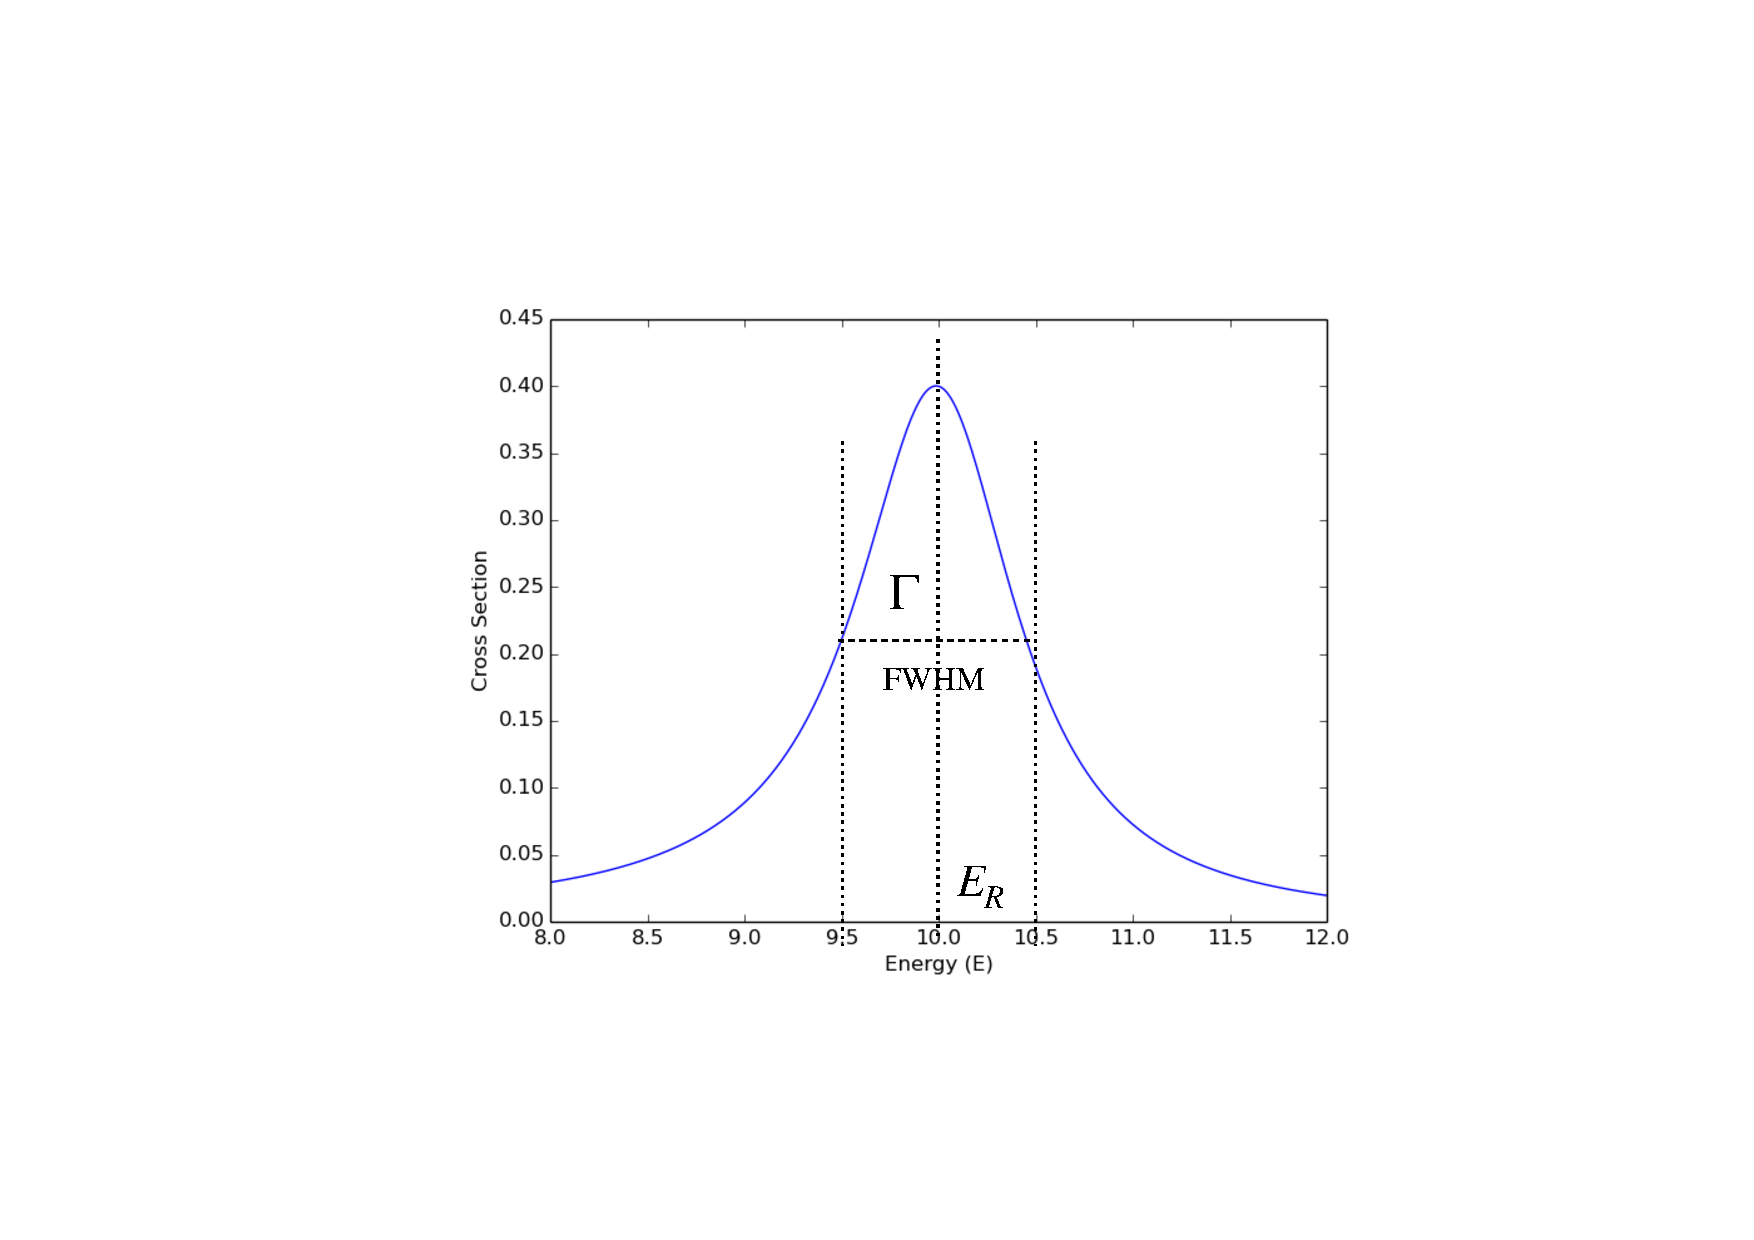
\includegraphics[width=0.5\textwidth]{BW}
\caption{Illustration of the cross section distribution as a function of energy, for a resonant process.}  \label{fig:BW}
\end{figure}

\section{Back to the plane wave model}
This transition can be treated similarly to the
dumped harmonic oscillator. Let us consider the wave function of a free
particle\footnote{We'll keep $\hslash$ in these equations.} (plane wave),
\[\psi(\vec{x},t) = \psi(\vec{x})e^{-\frac{iEt}{\hslash}}\].

As done for the dumped oscillator, let's include an imaginary term at
the exponential, by substituting $E$ with
\[E = E_0 -i\frac{\Gamma}{2},\]
which implies that $\Gamma$ has the
same units as energy. We chose the factor \(2\) in order to have a convenient expression of the probability of finding the particle in a given point, as
\begin{eqnarray}
  \label{eq:decay-0.5}
  \psi(\vec{x},t) &=& \psi(\vec{x})e^{-\frac{iE_0t}{\hslash}}\,e^{-\frac{\Gamma t}{2\hslash}},\\
  \abs{\psi(\vec{x},t)}^2 &=& \abs{\psi(\vec{x})}^2e^{-\frac{\Gamma t}{\hslash}}.
\end{eqnarray}

Let's now consider the decay of $N$ particles from the probabilistic
point of view. We introduce the mean lifetime of a particle $\tau$,
under the following hypotheses:\footnote{In other words, we are assuming that particle decays are Poisson processes.}
\begin{itemize}
\item the decay probability is an intrinsic property of a given particle;
\item the ratio between decay probability and time does not depend on
  time;
\item given a set of \(N\) particles, the decay probability of each single
  particle does not depend on \(N\).
\end{itemize}

Under these hypotheses, the differential of the probability (i.e. the probability of a particle to decay in a time \(dt\)) can be
written as:
\begin{equation}
  \label{eq:decay1}
  dp = \lambda dt,
\end{equation}
where $\lambda=1/\tau$ is the \emph{decay constant}.  If we now take back the full
set of particles, from a statistical point of view the probability
that, at the time $t$, $dN$ of them has decayed, is:
\[dp = -\frac{dN}{N(t)}\] in which we used $N(t)$ to denote the number
of particles at time $t$. Using Eq. \eqref{eq:decay1} we can write
\begin{eqnarray*}
  -dN &=& \lambda N(t) dt,\\
  -\qq{\ln N}^t_{t_0} &=& \lambda t - \lambda t_0,
\end{eqnarray*}
and if we call $N(0) = N_0$, and with no loss of generality set $t_0 = 0$,  we get
\[N(t) = N_0 e^{-\lambda t}.\]

The mean lifetime of a particle can be computed from the probability
of not having decayed after a time $t$,
\[\mathcal{P}(t) = \frac{N(t)}{N_0} = e^{-\lambda t},\]
as
\begin{eqnarray*}
  \tau \equiv \avg{t}  &\equiv& \frac{\int_0^\infty t \mathcal{P}(t)\,dt}{\int_0^\infty \mathcal{P}(t)\,dt}\\
                   &=&  \frac{\int_0^\infty t e^{-\lambda t}\,dt}{\int_0^\infty e^{-\lambda t}\,dt}\\
                   &=&  \frac{\int_0^\infty t e^{-\lambda t}\,dt}{-\frac{1}{\lambda}\qq{e^{-\lambda t}}_0^\infty}\\
                   &=&  \lambda \int_0^\infty t e^{-\lambda t}\,dt.
\end{eqnarray*}
We can solve this integral by parts. First, identify $u(x) \equiv x$ and $dv(x)/dx \equiv e^{-x}$, i.e.
\[v(x) = -e^{-x}.\]
Since $u\,dv = d(uv) - v\,du$, we can write
\[\tau = \cc{\qq{-xe^{-x}}_0^\infty + \int_0^\infty e^{-x}\,dx}\frac{1}{\lambda}.\]
Now, considering that
\[\lim_{x\rightarrow\infty}\frac{e^x}{x} = +\infty\]
and that \[\lim_{x\rightarrow\infty}xe^{-x} = 0\] we get
\[\tau = \frac{1}{\lambda}\qq{-e^{-x}}_0^\infty = \frac{1}{\lambda},\]
which defines the mean lifetime of a particle as
\[\tau = \frac{1}{\lambda}.\]

Some useful definitions arise from the concept of mean lifetime: the \emph{activity} of a radioactive source at a given time is defined as
\[A(t) = \lambda N(t) = \lambda N_0 e^{-\lambda t},\]
and the \emph{half-life} \(T_{1/2}\) is defined as the time needed before half of a set of $N$ particles has decayed: in formulas,
\[N(T_{1/2}) = \frac{N_0}{2}\],
which gives
\[e^{-\lambda T_{1/2}} = \frac{1}{2}\]
i.e.
\[T_{1/2} = \tau \ln 2.\]

We can now put in a relation the exponential law for the decay probability and the one obtained from equation \ref{eq:decay-0.5}:
\[e^{-\frac{\Gamma t}{\hslash}} = e^{-\frac{t}{\tau}},\]
which leads to
\[\Gamma = \frac{\hslash}{\tau}.\]
This equation can be seen as consistent with Heisenberg's uncertainty principle for time and energy measurements.

\section{Breit-Wigner formula and width of a resonance}
As for the dumped harmonic oscillator, it is possible to compute the wave function as a function of energy, py performing the Fourier--transform
\[ \chi (E) = \frac{1}{\sqrt{2\pi}}  \int_{-\infty}^\infty \psi(\vec{x},t)e^{i\frac{Et}{\hslash}}\,dt.\]
If we assume $\psi(\vec{x},t) = 0$ for $t<0$, we can write
\[ \chi (E) = \frac{\psi(0)}{\sqrt{2\pi}}  \int_0^\infty e^{-i\rr{E_0-i\frac{\Gamma}{2}}\frac{t}{\hslash}}e^{i\frac{Et}{\hslash}}\,dt,\]
and we have
\begin{eqnarray*}
 \chi (E) &=& \frac{\psi(0)}{\sqrt{2\pi}}  \int_0^\infty e^{\qq{i\rr{E-E_0}-\frac{\Gamma}{2}}\frac{t}{\hslash}}\,dt\\
          &=& \frac{\psi(0)}{\sqrt{2\pi}} \frac{ -i\hslash}{\rr{E-E_0}+i\frac{\Gamma}{2}} \qq{ e^{\qq{i\rr{E-E_0}-\frac{\Gamma}{2}}\frac{t}{\hslash}}}_0^\infty \\
          &=& \frac{\psi(0)}{\sqrt{2\pi}} \frac{ i\hslash}{\rr{E-E_0}+i\frac{\Gamma}{2}}.
\end{eqnarray*}
Then, the probability of having a particle with energy $E$ is
\[\mathcal{P}(E) \propto \abs{\chi(E)}^2 = \frac{\abs{\psi(0)}^2}{2\pi} \frac{ \hslash^2}{\rr{E-E_0}^2+\frac{\Gamma^2}{4}},
\]
which is known as the \emph{Breit--Wigner formula},
\[\mathcal{P}(E) \propto \frac{1}{\rr{E-E_0}^2 + \frac{\Gamma}{4}},\]
which has the characteristic shape of a resonance, also known as a \emph{Lorentian} function. Here $\Gamma$ represents the full-width at half-maximum (FWHM) of this distribution.

\begin{figure}
%  \centering
  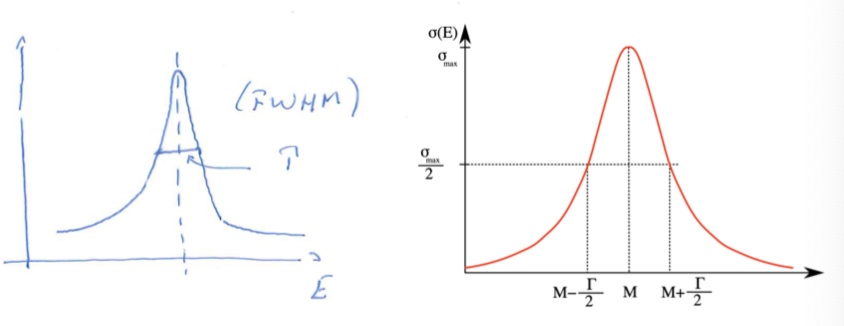
\includegraphics[width=0.8\textwidth]{decay1}
\caption{Graphic of the Laurentian form of $\mathcal{P}(E)$}  \label{fig:decay1}
\end{figure}

This representation of the particle in the energy Fourier--space highlights the relationship between its decay width and  its decay time.

If we collide two particles \(A\) and \(B\) that produce a given final state, and measure the corresponding interaction cross-section as a function of the center-of-mass energy, we may observe that the cross section shows ``peaks'' (i.e. resonances) for certain energy values, in a very similar way as harmonic oscillators do when the frequency of an external force varies. In particle physics processes, the presence of a peak is associated with the formation of a quantum state, which can be a particle or an excited state of a composite system.

For example, the reaction $A + B \to C +D+X$, can happen through an intermediate state, such as
\[ A+B \to Y+ X \to C+D+X,\]
where $Y$ decays to $C+D$.\footnote{A process like this is often also indicated as
\[
A+B\to Y(\to C+D) + X.
\]
}

Experimentally, one can measure the presence of resonances by measuring, for different values of the center-of-mass energy \(\sqrt{s}\) of the system \(A+B\) (which is obtained, for example, by measuring the energy of colliding particle beams in an accelerator), the cross--section of production of the final state \(C+D+X\). When the center-of-mass energy approaches the mass of the intermediate state \(Y\), \(\sqrt{s}\approx m_Y\), one will observe a resonant increase in the cross--section. The full-width at half-maximum of the distribution of the cross--section as a function of \(\sqrt{s}\) will be \(\Gamma=\hslash/\tau\).

Equivalently, one can observe the presence of resonances also by measuring the \emph{invariant mass} distribution of the system \(C+D\). This distribution will show a peak when the invariant mass equals to \(m_Y\). This is the way the Higgs boson \(H\) was discovered in 2012 by the ATLAS and CMS experiments at the Large Hadron Collider: we observed for example an increase in the number of events with two photons, in correspondence of an invariant mass of the di-photon system of about \SI{125}{GeV/c^2}.

\section{Radioactive decays}\label{sec:radioactivedec}
Historically, three main different kinds of radioactive emission have been observed:
\begin{itemize}
\item alpha radiation: with the emission of $\alpha$ particles (i.e. helium nuclei), positively charged ($z = +2$ in units of $e$) and a mass of $3.726\,\giga\electronvolt$: if we consider a nucleus \(A\) with \(Z\) protons and \(N\) neutrons, it will transform in the nucleus \(A'\) via the process
\[
A(Z,N)\to A'(Z-2, A-4) + \alpha;
\]
\item beta radiation: corresponding to the emission of an electron or of a positron (historically also called as ``beta particle''), with mass equal to $m_e = 0.511\,\mega\electronvolt$; one can have one of the two\footnote{One could observe that the \emph{electron capture} process \[A(Z,N)+e^-\to A(Z-1,N+1)+\nu_e\] is effectively described in the same way as the beta decay, as the involved particles and the underlying interaction are related.} processes\footnote{Note that the process with the emission of a positron would not be allowed in vacuum, as \(m_p<m_n\). It can only happen if another particle, like the nucleus, can ensure energy-momentum conservation.}
\begin{align*}
A(Z,N)\to A'(Z+1, A-1) + e^- + \bar{\nu}_e,\\
A(Z,N)\to A'(Z-1, A+1) + e^+ + \nu_e,
\end{align*}
which are called \(\beta^-\) and \(\beta^+\) decays, respectively;
  \item gamma radiation (emission of a photon), neutral and massless, due to the de-excitation of a nucleus via a process of the kind
  \[
A(Z,N)^*\to A(Z, N) + \gamma;
\]
\end{itemize}
Note that gamma radiation does not alter the chemical properties of the nucleus (we have \(A\) both before and after the gamma decay).

The typical momenta measured in these processes is around $1\,\mega\electronvolt$ for beta and gamma emissions and around $200\,\mega\electronvolt$ for alpha. The underlying process which is responsible for these radioactive decays is in general the emission of a particle in a transition between two nuclear quantum states (from a less bound to a more bound state).

Let's consider the kinematics of the decay process
\[N\rightarrow D_1 + D_2.\]
In the reference frame of the decaying nucleus, the conservation of energy implies
\[E_N = m_Nc^2 = m_{D_1}c^2 + K_{D_1} + m_{D_2}c^2 + K_{D_2},\]
where $K_{D_i}$ denotes the kinetic energy of the i-th nucleus. Defining $Q = m_Nc^2 - m_{D_1}c^2 -  m_{D_2}c^2$ as \emph{disintegration energy},  energy conservation implies that \[Q =  K_{D_1} + K_{D_2}\] defines the amount of kinetic energy held by the decay products (also called ``fragments''). In general, the decay is kinematically allowed only if $Q> 0$.

We can estimate \(Q\) for alpha and beta decays:
\begin{itemize}
\item for alpha decays, given an initial nucleus with $A$ and $Z$,
  \[Q = M(A,Z)c^2 - M(A-4,Z-2)c^2 -M_{\alpha};\]
\item for the \(\beta^-\) decay (i.e. the process with the emission of an electron),
  \[Q = M(A,Z)c^2 - M(A,Z+1)c^2 -m_ec^2;\]
\item for the \(\beta^+\) decay (i.e. the process with the emission of a positron),
  \[Q = M(A,Z)c^2 - M(A,Z-1)c^2 -m_ec^2.\]
\end{itemize}

Let's find an expression for the kinetic energy of the fragments in the reference frame of the initial nucleus: starting from the conservation of momentum,
\begin{eqnarray*}
\vec{P}_N^\text{tot} &=& 0,\\
  P_{D_1} &=& P_{D_2},
\end{eqnarray*}
we can write the energy of the daughter particle \(1\) as
\begin{eqnarray*}
  \sqrt{m_{D_1}^2+P_{D_1}^2} &=& m_{D_1} + K_{D_1},\\
  m_{D_1}^2+P_{D_1}^2 &=& m_{D_1}^2 + K_{D_1}^2 +2m_{D_1}K_{D_1},\\
  P_{D_1}^2 &=& K_{D_1}^2 +2m_{D_1}K_{D_1}\\
  &=& K_{D_2}^2 +2m_{D_2}K_{D_2},
\end{eqnarray*}
and using the definition of \(Q\) we can write
\begin{eqnarray*}
  K_{D_1}^2 - K_{D_2}^2 &=& \rr{K_{D_1}-K_{D_2}}\rr{K_{D_1}+K_{D_2}}\\
  &=& Q\rr{K_{D_1}-K_{D_2}},
\end{eqnarray*}
so that
\begin{eqnarray*}
K_{D_1}^2-K_{D_2}^2 &=& 2m_{D_2}K_{D_2}-2m_{D_1}K_{D_1},\\
Q\rr{K_{D_1}-K_{D_2}} &=& 2m_{D_2}K_{D_2}-2m_{D_1}K_{D_1},\\
QK_{D_1}+2m_{D_1}K_{D_1} &=& QK_{D_2}  + 2m_{D_2}K_{D_2},\\
\frac{K_{D_1}}{K_{D_2}} &=& \frac{2m_{D_2}+Q}{2m_{D_1}+Q}  
\end{eqnarray*},
and we can solve for the kinetic energy of particle \(1\), as
\begin{eqnarray*}
  K_{D_1} &=& \frac{2m_{D_2}+Q}{2m_{D_1}+Q} K_{D_2}\\
  &=& \frac{2m_{D_2}+Q}{2m_{D_1}+Q} \rr{Q-K_{D_1}}\\
  K_{D_1}\rr{1+\frac{2m_{D_2}+Q}{2m_{D_1}+Q}} &=& \frac{2m_{D_2}+Q}{2m_{D_1}+Q}Q\\
\end{eqnarray*}
which becomes
\[K_{D_1}\qq{2\rr{m_{D_1}+m_{D_2} + Q}} = \rr{2m_{D_2} +Q}Q,\]
i.e.
\[K_{D_1} = \frac{2m_{D_2}+ Q}{2\rr{m_{D_1}+m_{D_2}+Q}}Q,\]
and a corresponding analogous relation for $K_{D_2}$,
\[K_{D_2} = \frac{2m_{D_1}+ Q}{2\rr{m_{D_1}+m_{D_2}+Q}}Q.\]
In other words, if we know the \emph{\(Q\)-value} of a decay and the masses of the daughter particles, we can immediately know the kinetic energy of the daughter particles.

%The measurement units of radioactivity are briefly discussed in Chapter~\ref{chap:units}.

\section{Natural and secular equilibrium}
In many different cases the number of radioactive atoms in a system can increase with time. One example is the process
\[ n + ^{14}\text{N} \rightarrow ^{14}\text{C} +  p,\]
in which a nitrogen atom becomes a radioactive isotope of carbon (i.e. same atomic number but different mass number as carbon). This reaction happens in the high atmosphere, in which a flux of free neutrons is created by the scattering of cosmic rays with air molecules. Neutrons produced in this way are slowed down due to collisions with air molecules and, after their velocity has been reduced enough, they are captured by nitrogen atoms.
The reaction in which an incoming particle collides with an atomic nucleus, producing lighter particles in the final state (like protons, neutrons, alpha, etc...)  is called \emph{spallation}. An increased number of radioactive elements can also be the consequence of the activity of a nuclear reactor, a particle accelerator or the presence of a chain decay reaction.

We can write the variation in number of  radioactive atoms (particles, in the following) in all these cases as the sum of a term which corresponds to an increase in number of particles, and a term which takes into account their decay:
\begin{equation}
  \label{eq:decay2}
  \frac{dN}{dt} = R -\lambda N,
\end{equation}
where \(R>0\) and \(\lambda=1/\tau\) is the decay constant of the considered particles. The number of particles reaches equilibrium when
\[R = \lambda N,\]
or
\[N = \frac{R}{\lambda}.\]

Equation \ref{eq:decay2} can also be integrated between a time \(0\) and \(t\),
\begin{eqnarray*}
  \frac{dN}{dt} &=& -\lambda\rr{N-\frac{R}{\lambda}},\\
  \frac{dN}{N-\frac{R}{\lambda}} &=& -\lambda\,dt\\
  \qq{\ln\rr{N-\frac{R}{\lambda}}}_{N_0}^{N(t)} &=& e^{-\lambda t},
\end{eqnarray*}
which gives the following expression for $N(t)$,
\[N(t) = \frac{R}{\lambda} +\rr{N_0 -\frac{R}{\lambda}}e^{-\lambda t},\]
where we called as before \(N_0=N(0)\).

What happens if we have a decay chain
\[S_1 \rightarrow S_2 \rightarrow S_3,\]
in which $S_1$ and $S_2$ are radioactive particles, with decay constants $\lambda_1$ and $\lambda_2$, and \(S_3\) is a stable particle? The corresponding populations evolve according to the laws
\begin{equation}
  \label{eq:decay3}
  \frac{dN_1}{dt} = -\lambda_1 N_1,
\end{equation}
\begin{equation}
  \label{eq:decay4}
  \frac{dN_2}{dt} = \lambda_1 N_1-\lambda_2 N_2,
\end{equation}
\begin{equation}
  \label{decay5}
  \frac{dN_3}{dt} = \lambda_2 N_2,
\end{equation}
in which \eqref{eq:decay3} is the simple decay law, \eqref{eq:decay4} has the contribution of the decays of $S_1$ and \eqref{decay5} depends only on the amount of decays of $S_2$ (as $S_3$ is assumed to be non--radioactive).

Equation \eqref{eq:decay3} can be resolved as
\[N_1(t) = N_{1,0} e^{-\lambda_1 t}.\]
Equation \eqref{eq:decay4} can be resolved with the method of the variation of parameters, as it has the form
\[y'(t) + a(t)y(t) = f(t).\]
We must first find the solutions of the associated homogeneous equation,
\[y'(t) + a(t)y(t) = 0,\]
which are of the form
\[y(t) = K\exp\qq{-\int a(t)dt},\]
where \(K\) is a constant, and then look for a general solution
\[y(t) = K(t)\exp\qq{-\int a(t)dt}\].

In our case the homogeneous equation is:
\[\frac{dN_2}{dt} + \lambda_2N_2 = 0,\]
and the candidate solution is
\[N_2(t) = K(t)e^{-\lambda_2 t}.\]
We substitute it in Eq. \eqref{eq:decay4} and obtain
\begin{eqnarray*}
  \frac{dN_2}{dt} + \lambda_2 N_2 &=& \lambda_1 N_{1,0} e^{-\lambda_1 t},\\
  K'(t)e^{-\lambda_2 t} &=& \lambda_1 N_{1,0}e^{-\lambda_1 t},\\
  K(t) &=& \frac{\lambda_1}{\lambda_2 - \lambda_1}  N_{1,0} e^{\rr{\lambda_2-\lambda_1} t} + C,
\end{eqnarray*}
where \(C\) is a constant to determine. Therefore
\[N_2(t) = \frac{\lambda_1}{\lambda_2-\lambda_1} N_{1,0}e^{-\lambda_1 t} + Ce^{-\lambda_2 t}\],
and using $N_2(t=0) = N_{2,0}$ we can determine \(C\) as
\begin{eqnarray*}
  N_{2,0} &=& \frac{\lambda_1}{\lambda_2-\lambda_1} N_{1,0} + C,\\
  C &=&   N_{2,0} - \frac{\lambda_1}{\lambda_2-\lambda_1} N_{1,0}.
\end{eqnarray*}
Overall, we have
\[N_2(t) = \frac{\lambda_1}{\lambda_2-\lambda_1} N_{1,0} \rr{e^{-\lambda_1 t} - e^{-\lambda_2 t}} + N_{2,0}e^{-\lambda_2 t}.\]
We also obtain the following for $N_3(t)$:
\[N_3(t) = \int_0^t \lambda_2 N_2(t')dt'\].

Let's analyse the case in which $\lambda_2 \gg \lambda_1$, in which the term $e^{-\lambda_2 t}$ can be neglected: we have
\begin{eqnarray*}
  N_2(t) &=& \frac{\lambda_1}{\lambda_2} N_{1,0} e^{-\lambda_1 t}\\
  &=& \frac{\lambda_1}{\lambda_2} N_1(t),
\end{eqnarray*}
which can be written as
\[\lambda_1 N_1 = \lambda_2 N_2,\]
which means that the activities of $S_1$ and $S_2$ are equal. This leads to the concept of \emph{secular equilibrium},
\[\frac{N_2}{N_1} = \frac{\lambda_1}{\lambda_2} = \frac{\tau_2}{\tau_1}\]
where the relative concentration of different elements is equal to their mean lifetime ratio.

The concept of secular equilibrium applies also to longer decay chains of the form
\[S_1\rightarrow S_2\rightarrow S_3\rightarrow S_4\rightarrow S_5\rightarrow \dots \rightarrow  S_f,\]
for which one can write
\begin{eqnarray*}
  \frac{dN_1}{dt} &=& -\lambda_1 N_1\\
  \frac{dN_2}{dt} &=& \lambda_1 N_1 - \lambda_2N_2\\
  \frac{dN_k}{dt} &=& \lambda_{k-1} N_{k-1} - \lambda_kN_k\\
  \frac{dN_f}{dt} &=& \lambda_{f-1} N_{f-1}.
\end{eqnarray*}
If $\lambda_1 \ll \lambda_2,\lambda_3,\dots$, the equilibrium is reached:
\[\lambda_1 N_1 = \lambda_2 N_2 = \dots = \lambda_f N_f .\]

\section{Natural Radioactivity}
Secular equilibrium is at the basis of natural radioactivity, in which it's not uncommon to find nuclei with very long decay times ( $\tau \sim \mathcal{O}(10^9 \text{y})$). An example is uranium, $^{238}\text{U}$, whose decay chain leads to $^{210}\text{Pb}$ with a decay time of $4.5 \times 10^9\ \text{y}$.

Other examples are the alpha and beta chains of $^{232}\text{Th}$ (with $T_{1/2} = 1.4\times 10^{10}\ \text{y}$) and $^{235}\text{U}$ with $T_{1/2} = 7.5\times 10^{8}\ \text{y}$.\\

Other beta chains are  $^{10}\text{K}$ with $T_{1/2} = 1.3\times 10^{9}\ \text{y}$ or  $^{187}\text{Rb}$ with $T_{1/2} = 4.5\times 10^{10}\ \text{y}$.

\begin{figure}
%  \centering
  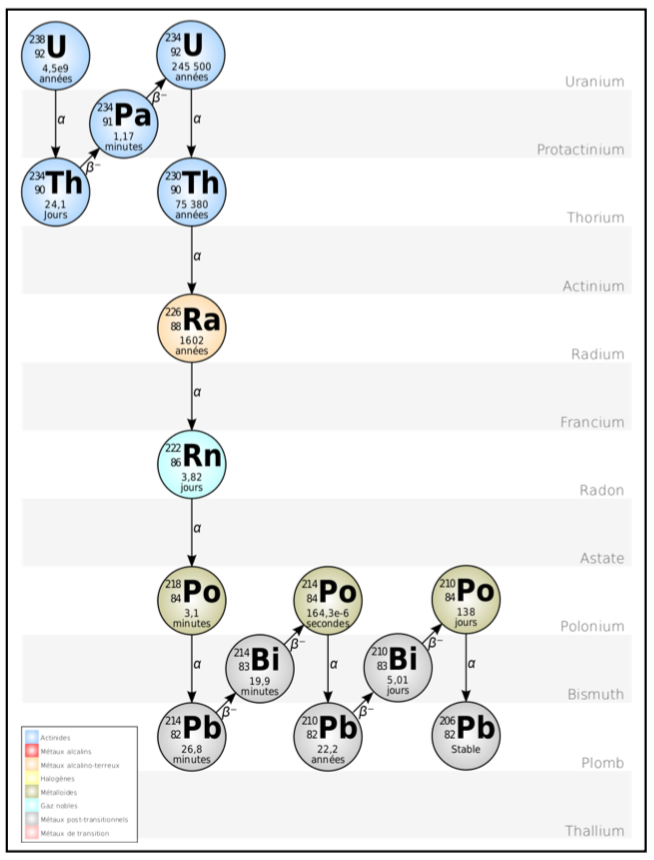
\includegraphics[width=0.8\textwidth]{decay2}
\caption{The decay chain started by \(^{238}U\). For each step, the kind of decay (in this case, alpha or beta) is also indicated.}  \label{fig:decay2}
\end{figure}



\begin{figure}
  \centering
  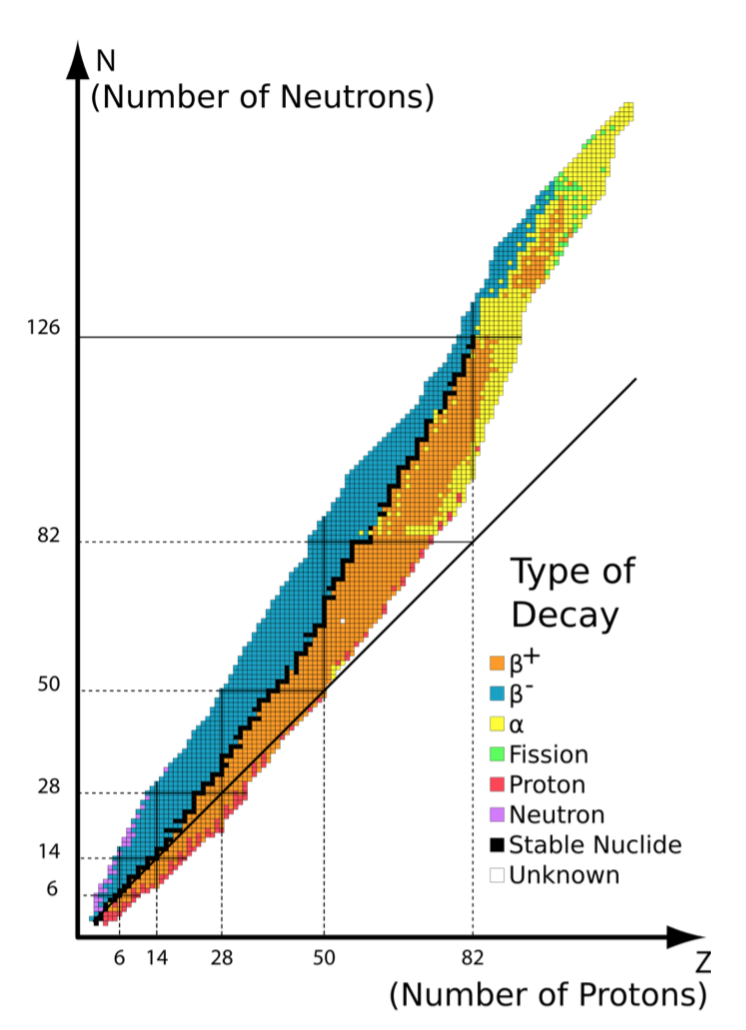
\includegraphics[width=0.5\textwidth]{decay3}
\caption{The Segré chart, which shows for each nucleus the type of decay it can occur as a function of its number of neutrons and protons. The dominant process which leads nuclei to the stability region is beta decay. The plot also shows that alpha decays happen only for high-mass nuclei. Remember that gamma decays do not affect the values of $A$ and $Z$, so they are not represented in this plot.}  \label{fig:decay3}
\end{figure}



\section{Alpha decays}
The radio-activity $\alpha$ can be interpreted as a form of nuclear fission
\begin{equation*}
    _{\tiny{Z}}^{\tiny{A}}\mbox{X} \rightarrow _{\tiny{Z-2}}^{\tiny{A-4}}\mbox{Y} + _{\tiny{2}}^{\tiny{4}}\mbox{He},
\end{equation*}
A known example is the process $^{\tiny{238}}\mbox{U} \rightarrow ^{\tiny{234}}\mbox{Th} + \alpha$, and the $\alpha$ particle is the helium nucleus.

As it can be seen in the Segré chart of Fig. \ref{fig:decay3},  $\alpha$ decays happen only for heavy nuclei, with $A > 210$. The process is a two-body decay, therefore the kinetic energy of the alpha particle is basically equal to the Q-value of the decay, $E_\alpha \sim Q_\alpha$. Experimentally one observes that, when different isotopes are considered, $Q$ varies following
\begin{equation*}
    Q = M(\mbox{X}) - M(\mbox{Y}) - M(\alpha).
\end{equation*}
Experiments also show a strong dependence of the life-time, $T_{1/2}$, on $Q$, following the empirical law
\begin{equation*}
    \ln T_{1/2} = a + \frac{b}{\sqrt{Q}},
\end{equation*}
which is called \emph{Geiger-Nuttal law}. This is illustrated in Fig. \ref{nuclear-physics-fig:4}.

As we have seen in Sec. \ref{sec:radioactivedec}, the kinetic energy of the \(\alpha\) particle is given by
\begin{equation*}
    K_\alpha = Q \frac{2M_{\mbox{Y}}+Q}{2(M_{\mbox{Y}}+m_{\alpha} + Q)},
\end{equation*}
which for example leads to 
\begin{equation*}
    ^{\tiny{208}}\mbox{Po}: \,\,\,Q = 5.2\,\mbox{MeV}\,\,\,T_{1/2} \sim 10^8 \mbox{s},
\end{equation*}
\begin{equation*}
     ^{\tiny{186}}\mbox{Po}: \,\,\,Q = 8.6\,\mbox{MeV}\,\,\,T_{1/2} \sim 10^{-5} \mbox{s}.
\end{equation*}
\begin{figure}[h]
    \centering
    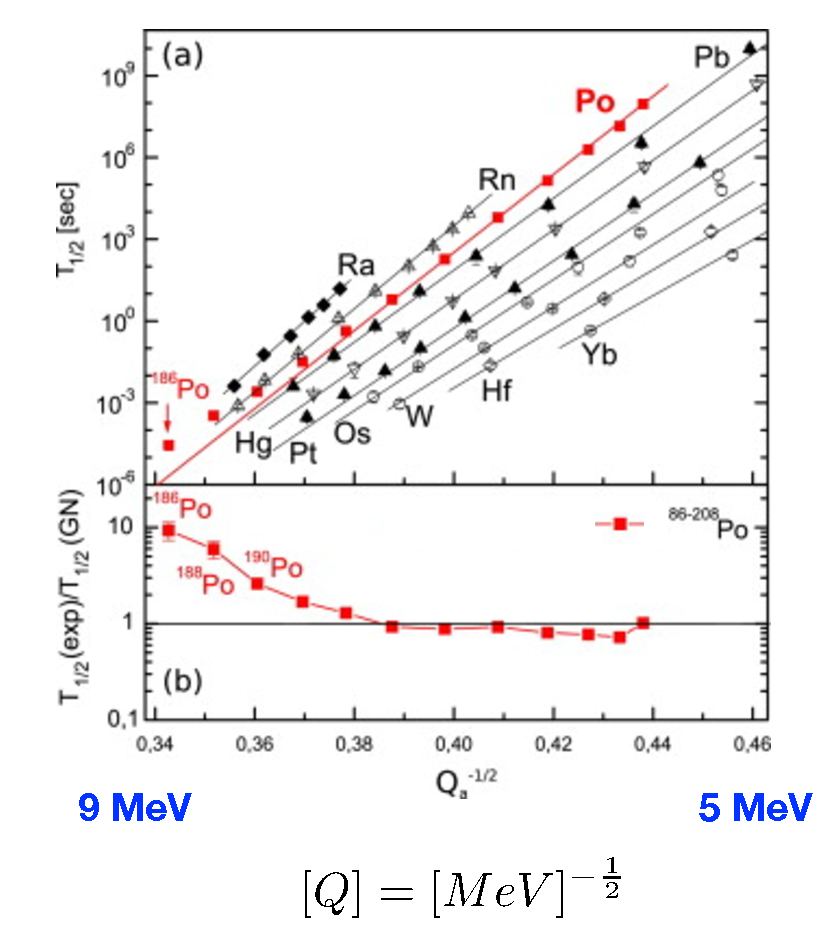
\includegraphics[scale=0.5]{Figures/nuclear-physics-fig4}
    \caption{Half time measurements for alpha decays of different isotopes. One observes an exponential distribution, with deviations at low $Q$}
    \label{nuclear-physics-fig:4}
\end{figure}

\subsection{Gamow's Model}
The Geiger-Nuttal law can be explained with a phenomenological model by Gamow. In this model, the nucleus is made of a $\alpha$ particle confined by a potential generated by the nucleus $N(A-4,Z-2)$. The $\alpha$ particle then has a non-zero probability to go through the potential barrier, as shown in Figure \ref{nuclear-physics-fig:5}.
\begin{figure}[h]
    \centering
    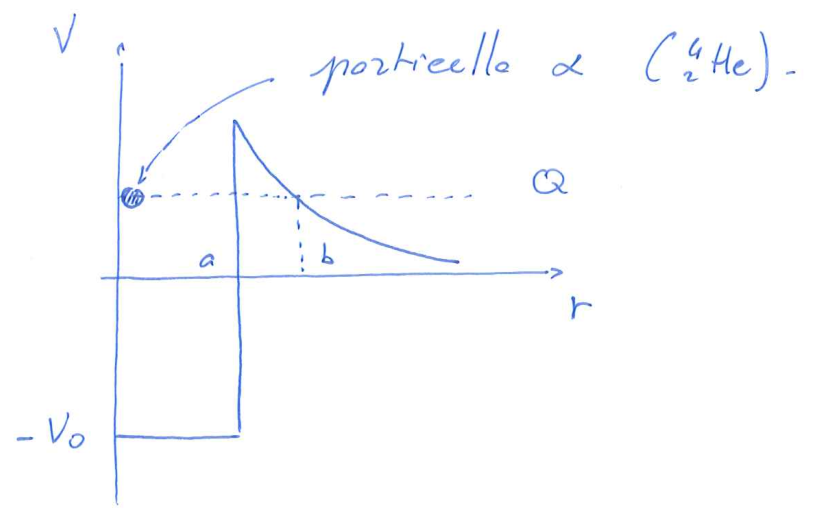
\includegraphics[scale=0.5]{Figures/nuclear-physics-fig5}
    \caption{Alpha particle in the potential generated by the \(N(A-4,Z-2)\) nucleus in Gamow's model.}
    \label{nuclear-physics-fig:5}
\end{figure}
Since the energy of the \(\alpha\) particle (of mass \(m\) is given by \(E=Q+V_0=\frac{1}{2}m v^2\), within the nucleus the $\alpha$ particle has a velocity
\begin{equation*}
    v = \sqrt{\frac{2(Q+V_0)}{m}},
\end{equation*}
and hits the potential barrier with a frequency given by $f = \frac{v}{2a}$. If $P$ is the tunneling probability, then the tunneling frequency (a good estimator of the alpha decay rate!) will be $fP$.

\subsection{Tunnel effect and potential barrier}
Let's try to evaluate the probability of transmission of a plane wave over a simple barrier show in Figure \ref{nuclear-physics-fig:6}.
\begin{figure}[h]
    \centering
    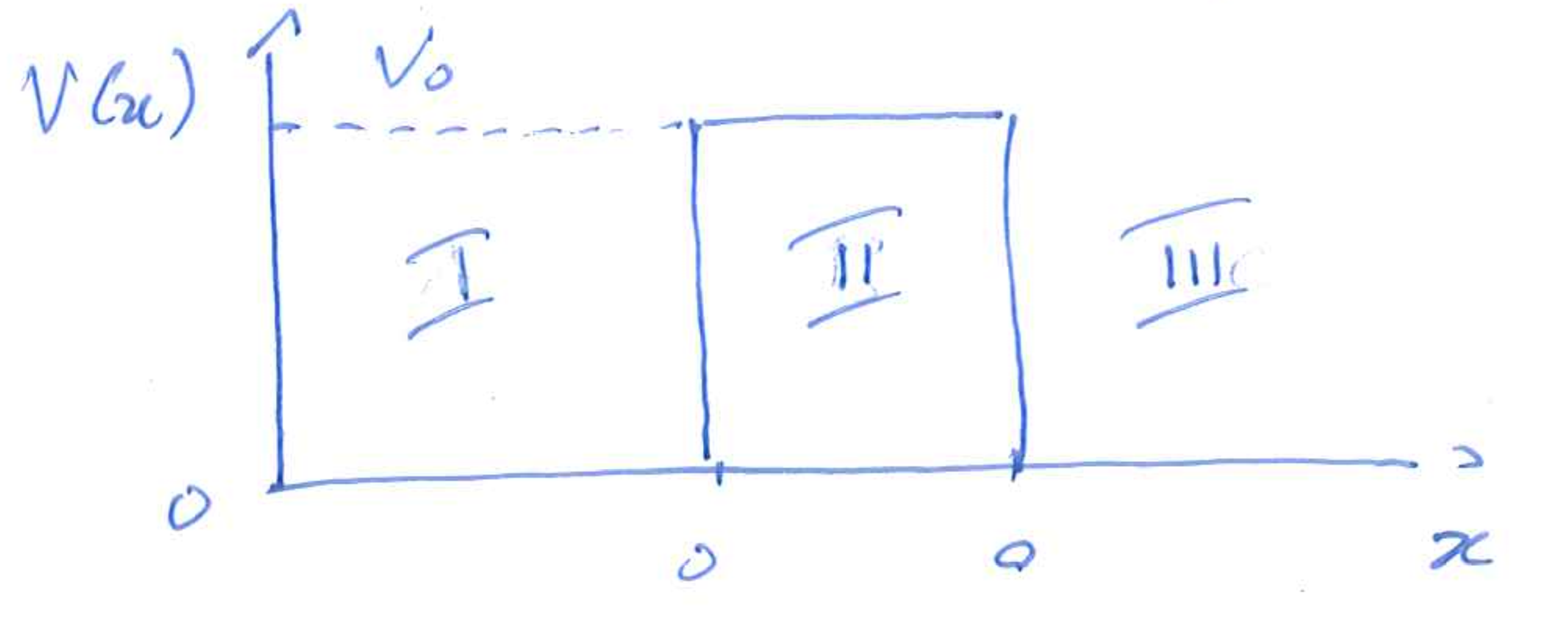
\includegraphics[scale=0.35]{Figures/nuclear-physics-fig6}
    \caption{Simple potential barrier, extending in one dimension from \(x=0\) to \(x=a\).}
    \label{nuclear-physics-fig:6}
\end{figure}
We can write the Schr\"odinger equation in the various regions as
\begin{equation*}
    [H_0 + V(x)]\psi = i\hslash\frac{\partial \psi}{\partial t}.
\end{equation*}

We look for solutions of the form
\begin{equation*}
    \psi (x,t) = \psi_{E}(x)e^{-iEt/\hslash}, % was with suffix varepsilon
\end{equation*}
which means we must solve the spatial equation
\begin{equation*}
    [H_0 + V(x)]\psi_E = E\psi_E,
\end{equation*}
which can be written in the three regions, using the free-particle hamiltonian $H_0=p^2/2m=-\hslash^2\nabla^2/2m$, as:
\begin{itemize}
    \item for regions I ($x<0$) and III ($x>a$), \begin{equation}
        \frac{d^2\psi_E}{dx^2} + \frac{2m}{\hslash^2}E\psi_E = 0;
    \end{equation}
    \item for region II ($0<x<a$),
    \begin{equation*}
        \frac{d^2\psi_E}{dx^2}+\frac{2m}{\hslash^2}(E-V_0)\psi_E = 0.
    \end{equation*}
\end{itemize}

If we define
\begin{equation*}
    k_0 = \sqrt{\frac{2m}{\hslash^2}(V_0 - E)},
\end{equation*}
and
\begin{equation*}
    k = \sqrt{\frac{2m}{\hslash^2}E},
\end{equation*}
it is easy to solve these Schr\"odinger equations. Note that, while \(k\) is a real number, \(k_0\) in general isn't: we will focus on the case \(E<V_0\), which corresponds to a particle whose energy is lower than the potential barrier. We are interested in knowing the tunneling probability of a particle whose energy is quite below the potential barrier. 

Let's look for solutions of the form
\begin{itemize}
    \item I ($x<0$): $\psi_E(x) = Ae^{ikx} + Be^{-ikx},$
    \item II ($0<x<a$): $\psi_E(x) = Ce^{k_0x}+De^{-k_0x},$
    \item III ($x>a$): $\psi_E(x)$ = $Fe^{ikx},$
\end{itemize}
which correspond to an incoming wave of amplitude $A$, a reflected wave of amplitude $B$ and a transmitted wave of amplitude $F$. The transmission factor is defined as
\begin{equation*}
    T = \frac{|F|^2}{|A|^2},
\end{equation*}
and can be calculated solving the Schr\"odinger equation. We can do it by imposing the continuity condition to the wave function and its first derivative:
\begin{itemize}
    \item in \(x = 0\) they imply
    \begin{equation*}
    \begin{split}
        & A+B = C+D,\\
        & ikA - ikB = k_0C -k_0D,
    \end{split}
    \end{equation*}
    and from the second equation we have
    \begin{equation*}
        A-B = -i\frac{k_0}{k}C + i\frac{k_0}{k}D,
    \end{equation*}
    which leads to
    \begin{equation*}
        \begin{split}
            & A = \frac{C}{2}\left(1+\frac{k_0}{ik}\right) + \frac{D}{2}\left(1-\frac{k_0}{ik}\right), \\
            & B = \frac{C}{2}\left(1-\frac{k_0}{ik}\right) + \frac{D}{2}\left(1+\frac{k_0}{ik}\right);
        \end{split}
    \end{equation*}
    \item in \(x = a\) we have
    \begin{equation*}
        \begin{split}
            & C e^{k_0a}+ De^{-k_0a} = Fe^{ika},\\
            & k_0Ce^{k_0a}-k_0De^{-k_0a} = ikFe^{ika},
        \end{split}
    \end{equation*}
    and from the second equation we have \begin{equation}
        Ce^{k_0a} - De^{-k_0a} = i\frac{k}{k_0} F e^{ika}.
    \end{equation}
    To solve this system of equations, we can write it conveniently in matrix form as
    \begin{equation*}
        \left( \begin{array}{cc}
        e^{k_0a} & e^{-k_0a} \\
        e^{k_0a} & -e^{-k_0a}
        \end{array} \right) 
        \left(\begin{array}{c}
        C \\
        D
        \end{array} \right) = 
        \left( \begin{array}{c}
        e^{ika} \\
        i\frac{k}{k_0}e^{ika}
        \end{array} \right) F,
    \end{equation*}
    and invert the matrix, 
    \begin{equation*}
        \left( \begin{array}{cc}
        e^{k_0a} & e^{-k_0a} \\
        e^{k_0a} & -e^{-k_0a}
        \end{array} \right)^{-1} 
        = \frac{1}{2}
        \left( \begin{array}{cc}
        e^{-k_0a} & e^{-k_0a}\\
        e^{k_0a} & -e^{k_0a}
        \end{array} \right),
    \end{equation*}
    so that we get
    \begin{equation*}
        \left( \begin{array}{c}
        C \\
        D
        \end{array} \right) 
        = \frac{1}{2}
        \left( \begin{array}{cc}
        e^{k_0a} & e^{-k_0a}\\
        e^{k_0a} & -e^{k_0a}
        \end{array} \right)
        \left( \begin{array}{c}
        e^{ika} \\
        i\frac{k}{k_0}e^{ika}
        \end{array}
        \right)F = \frac{1}{2}
        \left(
        \begin{array}{cc}
        e^{(ik-k_0)a} & \left(1+i\frac{k}{k_0}\right)F  \\
        e^{(ik+k_0)a} &\left(1-i\frac{k}{k_0}\right)F
        \end{array}
        \right).
    \end{equation*}
    \end{itemize}
    
We can express the solutions of \(A\) and \(B\) as a function of \(C\) and \(D\), as
 \begin{equation*}
    \left( \begin{array}{c}
    A \\
    B
    \end{array} \right) 
    = \frac{1}{2}
    \left( \begin{array}{cc}
    1+\frac{k_0}{ik} & 1-\frac{k_0}{ik}\\
    1-\frac{k_0}{ik} & 1+\frac{k_0}{ik}
    \end{array} \right)
    \left( \begin{array}{c}
    C \\
    D
    \end{array}
    \right),
\end{equation*}
so that it is immediate to substitute the expression calculated above to get 
\begin{equation*}
\begin{split}
     \left( \begin{array}{c}
    A \\
    B
    \end{array} \right) 
    & = \frac{e^{ika}}{4}F
    \left( \begin{array}{c}
    \left(1+\frac{k_0}{ik}\right)\left(1+\frac{ik}{k_0}\right)e^{-k_0a} + \left(1-\frac{k_0}{ik}\right)\left(1-\frac{ik}{k_0}\right)e^{k_0a}\\
    \left(1-\frac{k_0}{ik}\right)\left(1+\frac{ik}{k_0}\right)e^{-k_0a} + \left(1+\frac{k_0}{ik}\right)\left(1-\frac{ik}{k_0}\right)e^{k_0a}
    \end{array} \right) = \\
    & = \frac{e^{ika}}{4}F
    \left( \begin{array}{c}
    \left(2+i\left(\frac{k}{k_0}-\frac{k_0}{k}\right)\right)e^{-k_0a} + \left(2-i\left(\frac{k}{k_0}-\frac{k_0}{k}\right)\right)e^{k_0a}\\
    i\left(\frac{k}{k_0}+\frac{k_0}{k}\right)e^{-k_0a} - i\left(\frac{k}{k_0} + \frac{k_0}{k}\right) e^{k_0a}
    \end{array}
    \right) = \\
    & = \frac{e^{ika}}{4}F\left(
    \begin{array}{c}
    4\mbox{cosh}(k_0a) - 2i\frac{k^2-k_0^2}{k_0k}\mbox{sinh}(k_0a)\\
    -2i\frac{k^2+k_0^2}{k_0k}\mbox{sinh}(k_0a).
    \end{array}
    \right)
\end{split}
\end{equation*}
In other words, we have that
\begin{equation*}
    \left( \begin{array}{c}
    A \\
    B
    \end{array} \right) 
    = e^{ika}F
    \left( \begin{array}{c}
    \mbox{cosh}(k_0a)+\frac{k^2-k_0^2}{2ik_0k}\mbox{sinh}(k_0a)\\
    \frac{k^2+k_0^2}{2ik_0k}\mbox{sinh}(k_0a)
    \end{array} \right),
\end{equation*}
and the transmission coefficient is given by
\begin{equation*}
    \begin{split}
    T & = \frac{|F|^2}{|A|^2} = \frac{1}{\mbox{cosh}^2(k_0a) + \frac{(k^2-k_0^2)^2}{4k_0^2k^2} \mbox{sinh}^2(k_0a)} \\
    & = \frac{1}{1+\left[\frac{(k^2-k_0^2)^2}{4k_0^2k^2}+1\right] \mbox{sinh}^2(k_0a)},
    \end{split}
\end{equation*}
where we used the fact that $\mbox{cosh}^2 = 1+\mbox{sinh}^2$. After performing the sum at denominator can write
\begin{equation*}
    T = \frac{1}{1+\frac{(k^2+k_0^2)^2}{4k_0^2k^2} \mbox{sinh}^2(k_0a)},
\end{equation*}
and replacing the expressions of $k$ and $k_0$ we get
\begin{equation*}
     T = \frac{1}{1+\frac{V_0^2}{4E(V_0-E)} \mbox{sinh}^2(k_0a)}.
\end{equation*}
For the denominator, let's remember we are considering a particle which is quite deeply buried inside the potential, i.e. \(k_0a\gg 1\); we can therefore approximate
\begin{equation*}
    \mbox{sinh}^2(k_0a) = \frac{1}{4}\left(e^{2k_0a}-2+e^{-2k_0a}\right) \sim \frac{1}{4} e^{2k_0a},
\end{equation*}
and neglecting the first term in the denominator we have
\begin{equation*}
    T \sim \frac{16E(V_0-E)}{V_0^2}e^{-2k_0a}.
\end{equation*}
In the case in which $k \sim k_0$, then
\begin{equation*}
    \frac{16E(V_0-E)}{V_0^2} = \frac{16k_0^2k^2}{(k^2+k_0^2)^2} \sim 4,
\end{equation*}
therefore the probability to pass through the barrier will be
\begin{equation*}
    \mathcal{P} \sim 4e^{-2k_0a} = 4e^{-2a\sqrt{\frac{2m}{\hslash^2}(V_0-E)}}.
\end{equation*}


\subsection{Tunneling effect, generic potential}
For a generic potential \(V(r)\), the complete potential can be seen as a series of infinitesimal barriers of length \(dr\), where each of them has an associated probability to be passed through expressed by
\begin{equation*}
    d\mathcal{P} \propto e^{-2k_0dr} = e^{-2\sqrt{\frac{2m}{\hslash^2}(V(r)-Q)}dr},
\end{equation*}
where \(Q\) is the disintegration energy (Q-value), i.e. the total kinetic energy available to the particle.
The probability to go through the entire barrier is given by the product of the infinitesimal probabilities
\begin{equation*}
    \mathcal{P}=\prod^\infty d\mathcal{P}\propto e^{-2\int k_0 dr} = e^{-2\int_a^b\sqrt{\frac{2m}{\hslash^2}(V(r)-Q)}dr},
\end{equation*}
where the particle tunnels from \(r=a\) to \(r=b\), which represent the intersections between the horizontal line \(V=E\) and the potential \(V=V(r)\).
We can write
\begin{equation*}
    \mathcal{P} \propto e^{-2G},
\end{equation*}
where $G$ is the \emph{Gamow factor}
\begin{equation*}
    G = \int_a^b\sqrt{\frac{2m}{\hslash^2}(V(r)-Q)}dr.
\end{equation*}

For the Coulomb potential, represented in Figure \ref{nuclear-physics-fig:7}, we have
\begin{figure}[h]
    \centering
    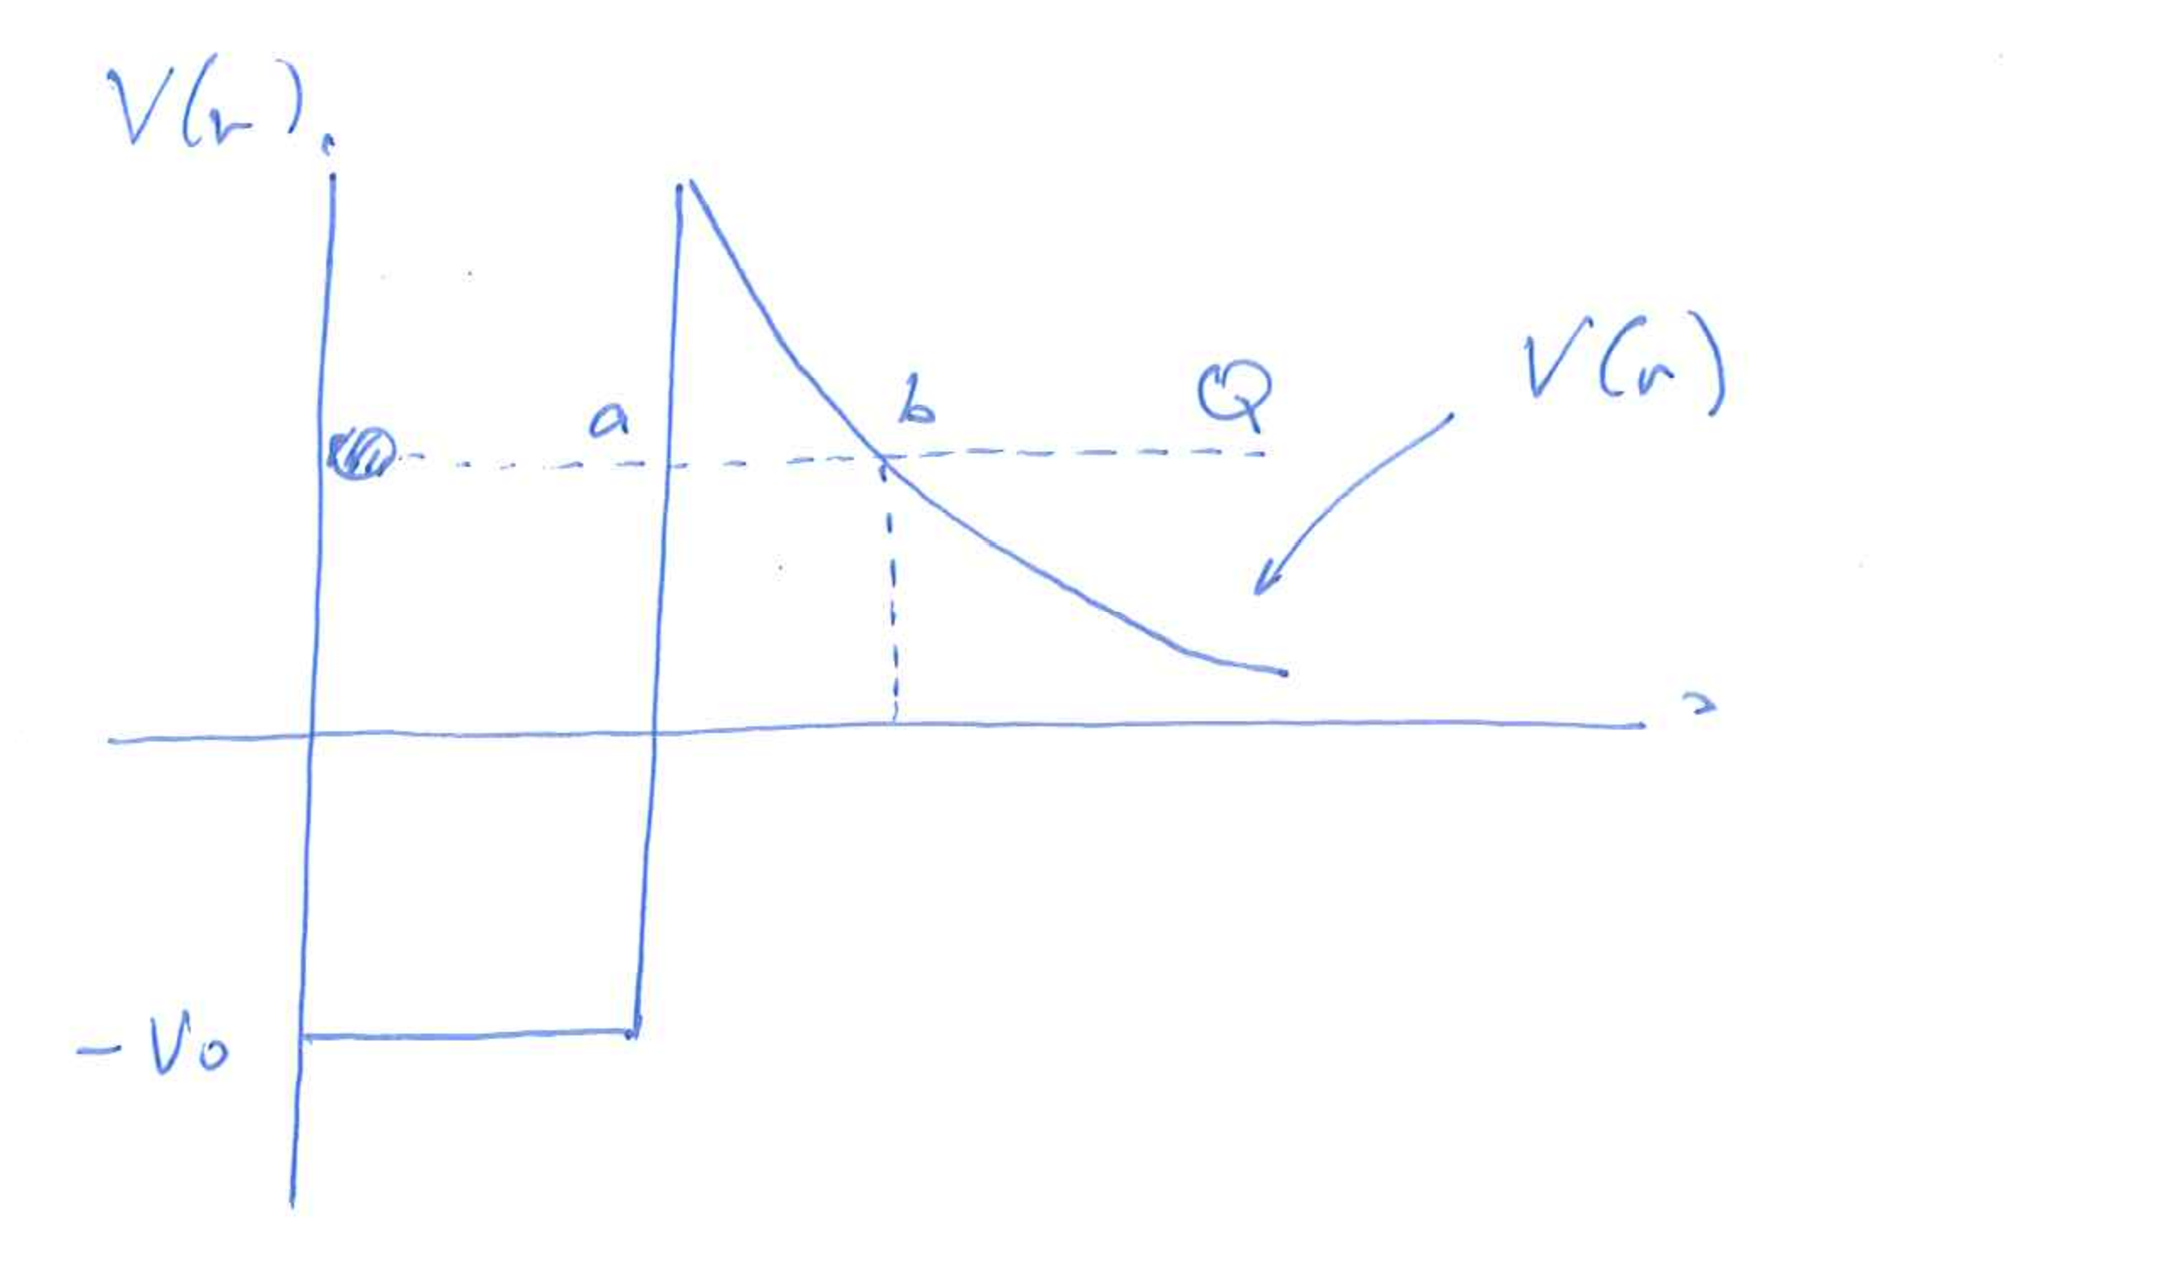
\includegraphics[scale=0.3]{Figures/nuclear-physics-fig7}
    \caption{Coulomb potential.}
    \label{nuclear-physics-fig:7}
\end{figure}
\begin{equation*}
    V(r) = \frac{2(\mbox{Z}-2)e^2}{4\pi\varepsilon_0 r} = \frac{2(\mbox{Z}-2)\alpha}{r}\hslash c,
\end{equation*}
and the total available energy can be obtained (see the figure) evaluating the potential for $r=b$:
\begin{equation*}
    Q = \frac{2(\mbox{Z}-2)\alpha}{b}\hslash c,
\end{equation*}
from which one has
\begin{equation}
    b = \frac{2(\mbox{Z}-2)\alpha}{Q}\hslash c.
\end{equation}
This gives us the possibility to calculate the Gamow factor for the Coulomb potential as
\begin{equation*}
    \begin{split}
        G & = \sqrt{\frac{2m}{\hslash^2}}\int_a^b\sqrt{\frac{(\mbox{Z}-2)2\alpha\hslash c}{r}-Q} dr = \sqrt{\frac{2mQ}{\hslash^2}}\int_a^b\sqrt{\frac{(\mbox{Z}-2)2\alpha\hslash c}{Qr}-1} dr = \\
        & = \sqrt{\frac{2mQ}{\hslash^2}}\int_a^b\sqrt{\frac{b}{r}-1}dr = \sqrt{\frac{2mQ}{\hslash^2}}\int_a^b\sqrt{\frac{b-r}{r}}dr = \sqrt{\frac{2mQ}{\hslash^2}}b\int_a^b\sqrt{\frac{1-r/b}{r/b}}d\left(\frac{r}{b}\right).
    \end{split}
\end{equation*}
This integral is not trivial, but from the table of integrals of irrational functions we get that
\begin{equation*}
    \int\sqrt{\frac{1-x}{x}}dx = \sqrt{x-x^2}+\mbox{arcsin}\sqrt{x}.
\end{equation*}
Therefore, with \(x=r/b\), 
\begin{equation*}
    \begin{split}
    G & = \sqrt{\frac{2mQ}{\hslash^2}}b\int_{a/b}^1\sqrt{\frac{1-x}{x}}dx = \sqrt{\frac{2mQ}{\hslash^2}}b\left[\left(\frac{\pi}{2}-\mbox{arcsin}\sqrt{\frac{a}{b}}\right)-\sqrt{\frac{a}{b}-\frac{a^2}{b^2}}\right] \\&= \sqrt{\frac{2mQ}{\hslash^2}}b \left[\mbox{arccos}\sqrt{\frac{a}{b}}-\sqrt{\frac{a}{b}-\frac{a^2}{b^2}}\right].
    \end{split}
\end{equation*}
If we chose $f\left(\frac{a}{b}\right) = \mbox{arccos}\sqrt{\frac{a}{b}}-\sqrt{\frac{a}{b}-\frac{a^2}{b^2}}$, given that $b = \frac{(\mbox{Z}-2)2\alpha\hslash c}{Q}$, then
\begin{equation*}
    G = \sqrt{\frac{2m}{\hslash^2Q}}\alpha\hslash c \left[2(\mbox{Z}-2) \right]f\left(\frac{a}{b}\right).
\end{equation*}

Taking all together, under the approximation that $k_0 \sim k$ we have that the decay rate can be written in terms of the velocity $v$ of the $\alpha$ particle as
\begin{equation*}
    fP = \frac{v}{2a}4e^{-2G} = \sqrt{\frac{2(Q+V_0)}{m}}\frac{2}{a}e^{-2G},
\end{equation*}
where \(Q+V_0\) is the energy of the \(\alpha\) particle (and \(V_0>0\) is the depth of the potential well).
Therefore, from the decay laws we have that the decay constant can be written as
\begin{equation*}
    \lambda = fP,
\end{equation*}
and therefore the mean lifetime  $\tau = \frac{1}{\lambda}$ is
\begin{equation*}
    \tau = \frac{1}{\lambda} = \sqrt{\frac{m}{2(Q+V_0)}}\frac{a}{2}e^{2G} = \sqrt{\frac{m}{2(Q+V_0)}}\frac{a}{2}e^{2\alpha\sqrt{\frac{2mc^2}{Q}}[2(\mbox{Z}-2)]f(a/b)}.
\end{equation*}
Therefore we obtain that
\begin{equation*}
    \ln\tau = \ln\left(\sqrt{\frac{m}{2(Q+V_0)}}\frac{a}{2}\right)+2\alpha\sqrt{\frac{2mc^2}{Q}}\left[2(\mbox{Z}-2)\right]f\left(\frac{a}{b}\right),
\end{equation*}
which explains the empirical Geiger-Nuttal's law introduced at the beginning of this section. The result of this calculation includes a slight dependence on \(Q\) from the constant factor $\ln\left(\sqrt{\frac{m}{2Q}}\frac{a}{2}\right)$, which leads to a family of functions in \(Z\).

The various possible transitions through $\alpha$ radiation emission reflect the excited states of the nuclei, as shown for example in Figure \ref{nuclear-physics-fig:8}. The $\alpha$ decays of the nuclei can lead to excited states, which then decay through the emission of $\gamma$ radiation to the fundamental states.



\begin{figure}
    \centering
    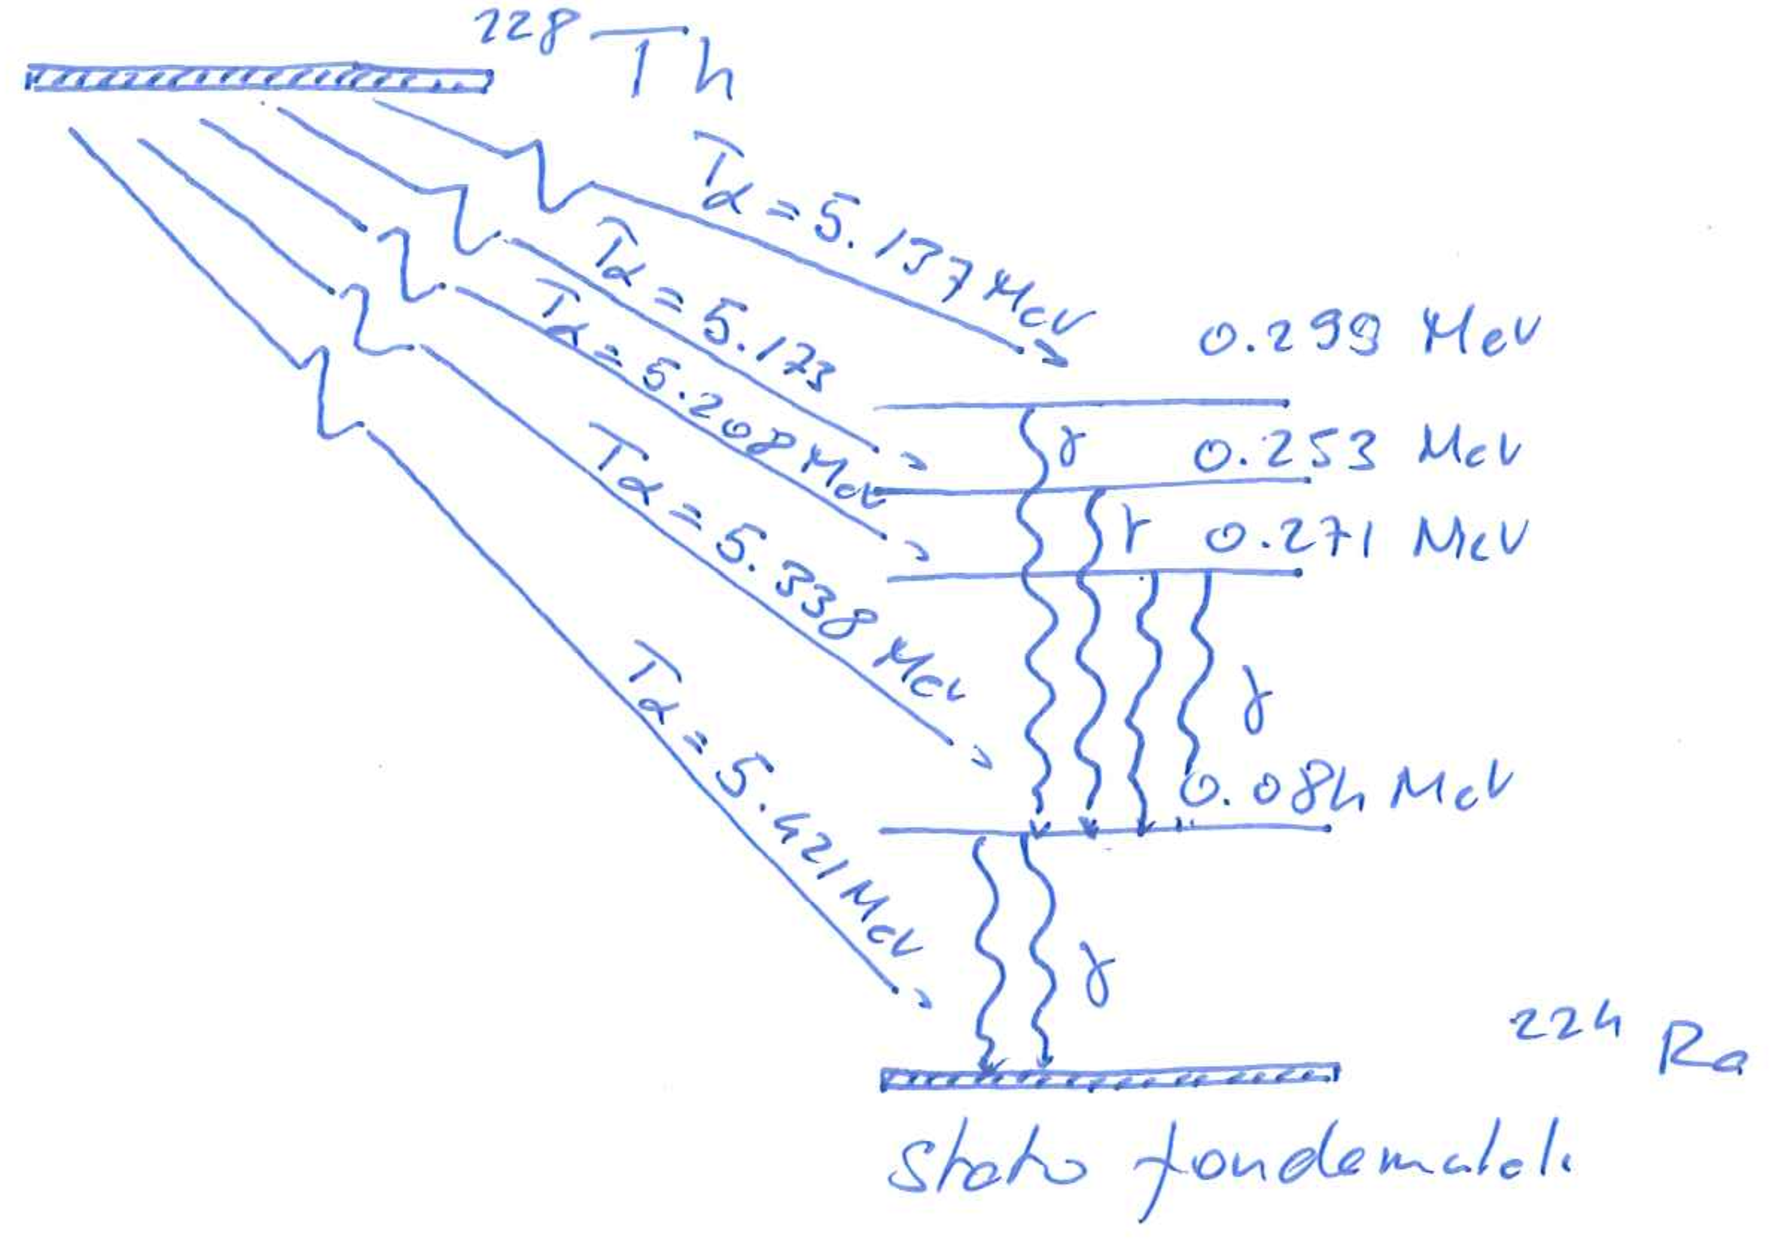
\includegraphics[scale=0.35]{Figures/nuclear-physics-fig8}
    \caption{Possible decays of  $^{\tiny{228}}\mbox{Th}$ through the emission of $\alpha$ particles.}
    \label{nuclear-physics-fig:8}
\end{figure}

\subsection{Interpretation}

The fact that the Gamow potential and tunnelling theory of the $\alpha$ radioactivity is very successful in reproducing the empirical Geiger-Nuttal's law shows that the nucleus can be well approximated by a 1D square well, which as we have seen in Chapter~\ref{scattering-2} can also be interpreted as a spherical 3D well with a short range of the size of the nucleus. Gamow's model, where the potential responsible for alpha decays is the Coulomb potential of the daughter nucleus, describes well experimental data. This corroborates the overall picture of Rutherford scattering which, until energy is sufficiently high, is insensitive to the effects of the strong force that binds the nucleus together. 

The Gamow potential picture can equivalently be used for an $\alpha$ particle scattering from outside the nucleus, as in the case of Rutherford scattering. Such scattering can be seen as happening off a static Coulomb potential until a sufficiently large energy is reached at which the $\alpha$ particle can be captured by the nucleus, as illustrated in Fig.~\ref{fig:RutherfordScatteringBreakdown}. This is precisely what was discussed in Section
~\ref{sec:RutherfordInterpretation}. 

\section{Beta decays and the Fermi theory}
\label{sec:FermiTheory}

The study of  $\beta$ radioactivity is crucial in developing an understanding of the structure of the nucleus. The development by Enrico Fermi in 1934 of a theory of the $\beta$ decays has incredibly far-reaching consequences.

We can start the description of the Fermi theory starting from the most basic observations of the $\beta$ radioactivity. The two essential experimental facts, as was discussed in Section~\ref{sec:DiscoveryRadioactivity}, are that the nature of the $\beta$ radiation is electrons or positrons and the $\beta$ decay spectrum is continuous.

This immediately brings serious interpretation challenges, which can be summarized as follows:

\begin{itemize}
    \item[-] contrary to the $\alpha$ decay, the $\beta$ decay process is not compatible with a two-body decay: the electron energy spectrum would in that case be close to a Dirac delta, and not a continuous distribution with an endpoint, as shown in Figure \ref{nuclear-physics-fig:17};
    \begin{figure}[h]
        \centering
        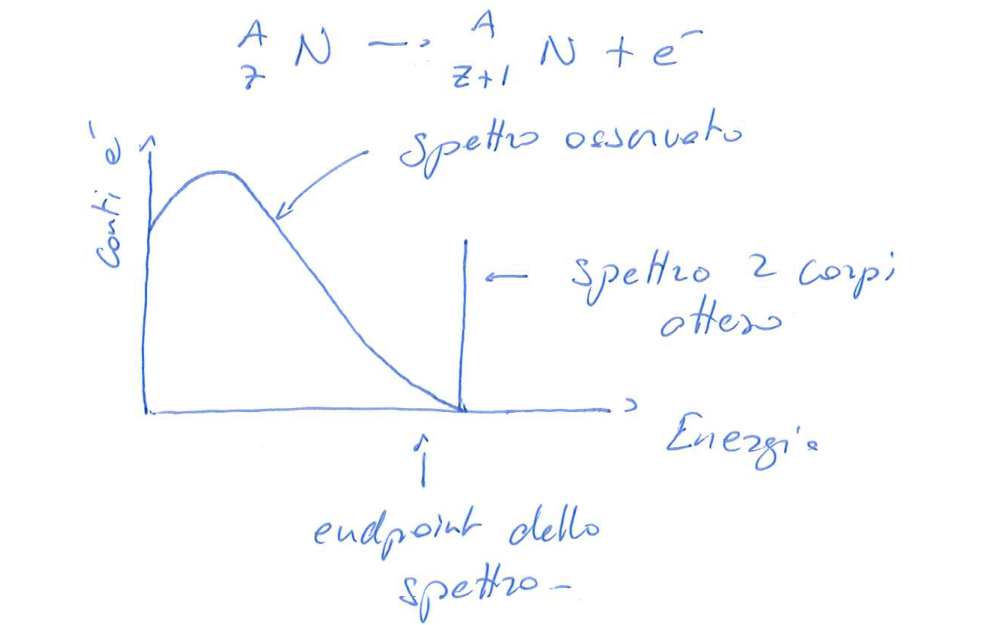
\includegraphics[scale=0.5]{Figures/nuclear-physics-fig17}
        \caption{Beta decay energy spectrum}
        \label{nuclear-physics-fig:17}
    \end{figure}
    
    \item[-] in the case of a two-body decay \(n\to p+e^-\), the total angular momentum would not be conserved, since the electron has spin $\frac{1}{2}$ and there are nuclear transitions which do not change the angular momentum;
    
    \item[-] how could one model the presence of electrons in the nucleus (in a similar way to $\alpha$ particles)? can there \emph{really} be electrons within the nucleus?
\end{itemize}

The consequences of these three challenges are:
\begin{itemize}
    \item the \emph{hypothesis} of a three-body decay, with the emission of an additional, neutral, ``invisible'' particle, which is extremely penetrating and interacts weakly (this is the hypothesis suggested by Pauli in 1932);
    \item this particle, named by Fermi the \textit{neutrino}, must have spin $1/2$, in order to address the total angular momentum conservation issue;
    \item the observation of the emission of this kind of particle \emph{at the same time} of the electron is of fundamental importance for the development of particle physics.
\end{itemize}
Since electrons do not take part in the interactions in the nucleus, Fermi hypothesised that they are \emph{created in pairs} together with a neutrino. The concept of pair-creation is a fundamental concept on which relativistic Quantum Field Theory is based -- which, differently from simple quantum mechanics, allows for the creation and destruction of new particles.

Several reactions and decays of $\beta$ type are observed:
\begin{itemize}
    \item $\beta^{-}$ decay: $_{\tiny{Z}}^{\tiny{A}}X \rightarrow _{\tiny{Z+1}}^{\tiny{A}}Y + e^-+\overline{\nu}_e$, which happens if 
    \begin{equation*}
        Q = \mbox{$M(A,Z) - M(A,Z+1) - m_e$} > 0
    \end{equation*}
    for the nuclei or if
    \begin{equation*}
        Q = m(\mbox{A,Z}) - m(\mbox{A,Z+1}) > 0
    \end{equation*} for the atoms.
    \item $\beta^+$ decay: $_{\tiny{Z}}^{\tiny{A}}X \rightarrow _{\tiny{Z-1}}^{\tiny{A}}Y + e^+(+\nu)$ which happens for \begin{equation*}
        Q = \mbox{$M(A,Z) - M(A,Z-1) - m_e$} > 0,
    \end{equation*} and therefore is not possible for an isolated proton.
    \item electronic capture: $p+e^- \rightarrow n+\nu_e$, is possible if \begin{equation*}
        Q = \mbox{$M(A,Z) + m_e - M(A,Z-1)$}
    \end{equation*}
\end{itemize}

\subsection{The Fermi theory}
\label{sec:FermiTheory}
In order to characterise \(\beta\) decays, we need to find an expression for the decay lifetime \(\tau=1/\lambda\) and the energy spectrum of the electron/positron in the final state.

We will use again  Fermi's golden rule, detailing the matrix element and the phase space. In this case we can no more consider that the electron (and the neutrino) which are emitted in decay are trapped into the nucleon before the emission, since the electron does not interact via the strong interaction. There must be a new type of interaction, as depicted in Figure \ref{nuclear-physics-fig:18}.
\begin{figure}[h]
    \centering
    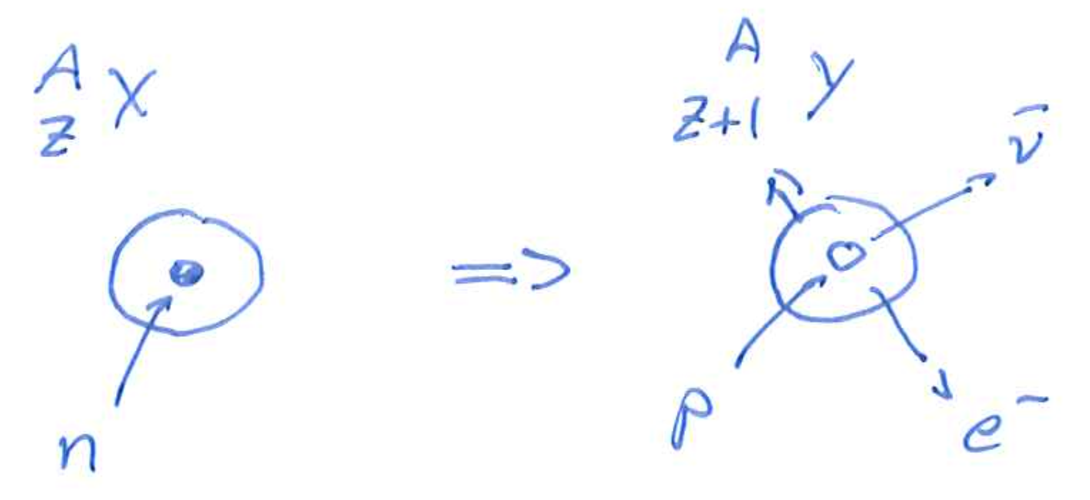
\includegraphics[scale=0.2]{Figures/nuclear-physics-fig18}
    \caption{Sketch of the interaction.}
    \label{nuclear-physics-fig:18}
\end{figure}

In 1934, Fermi proposed a theory which was able to explain the $\beta$ decay through a new type of interaction. It is based on the following hypotheses and it was an important idea towards the development of  quantum field theory:
\begin{itemize}
    \item in the $\beta$ decay we address the question on the nucleon decays as
    \begin{equation*}
        \beta^- :\,\,n\rightarrow p + e^- + \bar{\nu},
    \end{equation*}
    \begin{equation*}
        \beta^+ :\,\,p\rightarrow n + e^+ + \nu,
    \end{equation*}
    where the  \textit{anti-neutrino} is the anti-particle of the neutrino;
    \item the interaction must be able to create or absorb fermions;
    \item the new interaction is a short-range interaction, and in particular will be described as a \emph{contact interaction}.
\end{itemize}

Let us focus on the \(n\to p + e^- + \bar{\nu}_e\) process, where the neutron is at rest.
If we denote as $H_I$ the interaction hamiltonian responsible for this process, $H_I$ will need to absorb the neutron and emit a proton in a point $r_1$ and emit an electron and a neutrino in the point $r_2$, as depicted in Figure \ref{nuclear-physics-fig:19}. 
\begin{figure}[h]
    \centering
    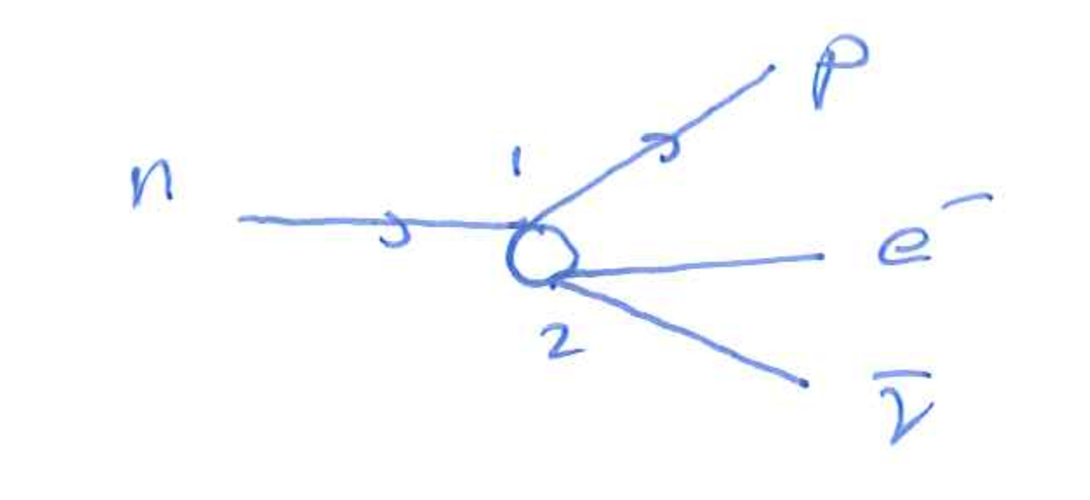
\includegraphics[scale=0.2]{Figures/nuclear-physics-fig19}
    \caption{The $\beta^{-}$ decay.}
    \label{nuclear-physics-fig:19}
\end{figure}
The matrix element of the decay can be written as
\begin{equation*}
    \langle pe^-\bar{\nu} | H_I | n \rangle = \int \psi_p^*(\Vec{r}_1)\psi_e^*(\Vec{r}_2)\psi_{\bar{\nu}}^*(\Vec{r}_2) H_I(\Vec{r}_1-\Vec{r}_2) \psi_n(\Vec{r}_1)\,d\Vec{r}_1d\Vec{r}_2,
\end{equation*}
where the double integral runs over all possible positions in space at which the proton is emitted, and at which the electron-antineutrino pair is emitted.

Assuming that this is a contact interaction means that the Hamiltonian can be written as the product of some constant \(g\) and a Dirac delta which imposes the ``contact'', i.e.
\begin{equation*}
    H_I(\Vec{r}_1 - \Vec{r}_2) = g\delta(\Vec{r}_1 - \Vec{r}_2).
\end{equation*}
Therefore, the matrix element of the decay simplifies as
\begin{equation*}
    \langle pe^-\bar{\nu} | H_I | n \rangle = g\int_V \psi_p^*(\Vec{r})\psi_e^*(\Vec{r})\psi_{\bar{\nu}}^*(\Vec{r})\psi_n(\Vec{r})\,d\Vec{r},
\end{equation*}
where the integral is extended to the whole nucleus where the \(\beta^-\) decay is happening.

Since the electron and the neutrino do not have nuclear interactions, we can assume that their wave functions are like the ones of free particles,
\begin{equation*}
    \psi_e^{-}(\Vec{r}) = \frac{1}{\sqrt{V}}e^{-i\Vec{p}_e\cdot\Vec{r}/\hslash},
\end{equation*}
\begin{equation*}
    \psi_{\bar{\nu}}(\Vec{r}) = \frac{1}{\sqrt{V}}e^{-i\Vec{p}_{\bar{\nu}}\cdot\Vec{r}/\hslash}.
\end{equation*}
We have chosen a normalisation such that
\begin{equation*}
    \int_V |\psi_{e^-,\nu}(\Vec{r})|^2\,d\Vec{r} = 1,
\end{equation*}
which means one particle for the volume \(V\). Therefore,
\begin{equation*}
    \psi_e(\Vec{r})\psi_{\bar{\nu}}(\Vec{r}) = \frac{e^{-i(\Vec{p}_e+\Vec{p}_{\nu})\cdot \Vec{r}/\hslash}}{V}.
\end{equation*}
We anticipate that, in the calculation of physical quantities such as decay rate and spectra, the volume \(V\) will cancel.

The electron and neutrino momenta in \(\beta\) decays are typically of the order of \(Q\approx \SI{1}{MeV/c}\), and we can assume that the wave functions have small variations within the integration volume, $r_0 \sim \SI{1}{fm}$. So we have
\begin{equation*}
    \frac{Qr_0}{\hslash} \sim \frac{1\,\mbox{MeV}\,\,\times\,\,1\,\mbox{fm}}{200\,\mbox{MeV}\cdot\mbox{fm}} \sim 10^{-2},
\end{equation*}
and we can expand in series
\begin{equation*}
\label{eq:LExpansion}
    e^{-i(\Vec{p}_e+\Vec{p}_{\bar{\nu}})\cdot\frac{\Vec{r}}{\hslash}} = 1 - \frac{(\Vec{p}_e + \Vec{p}_{\bar{\nu}})}{\hslash}\Vec{r} - \frac{1}{2}\left(\frac{(\Vec{p}_e+\Vec{p}_\nu)\cdot\Vec{r}}{\hslash}\right)^2 + \dots.
\end{equation*}
This is a very interesting point, since the values of the total angular momentum of the electron and neutrino system with respect to the nucleus will be small with respect to $\hslash$. This can be seen as the largest possible momentum in the decay will be $Q$ of the order of a \si{MeV}, with a radius of the order of a \si{fm} and $\hslash c \sim 197.3$~MeV~fm: this implies $\frac{(\Vec{p}_e + \Vec{p}_{\bar{\nu}})}{\hslash}\Vec{r} 
\sim 0.5\%$.

In the expansion we can consider  the first term alone, which is simply $1$, which yields the simplified expression for the Matrix element, which does not depend on the electron and neutrino momenta:
\begin{equation*}
    \langle f | H_I | i \rangle = \frac{g}{V}\int_{V}\psi_p^*(\Vec{r})\psi_{n}(\Vec{r})\,d\Vec{r},
\end{equation*}
or 
\begin{equation*}
    \langle f | H | i \rangle = \frac{g}{V}M_{fi}.
\end{equation*}

The interaction can be generalised to the decay of nuclei 
\begin{equation*}
    _{\tiny{Z}}^{\tiny{A}}N \rightarrow _{\tiny{Z+1}}^{\tiny{A}}Y + e^-+\bar{\nu},
\end{equation*}
with a zero-dimensional operator $O_x$ which can be chosen to reproduce experimental data. All the formalism is then equivalent in the two cases, as
\begin{equation*}
    \langle f | H_I | i \rangle = \frac{g}{V}\int_V \psi_{A,Z+1}^*(\Vec{r})O_x\psi_{A,Z}(\Vec{r})
\end{equation*}
can be written as
\begin{equation*}
\label{eq:ME-Fermi}
    \langle f | H_I | i \rangle = \frac{g}{V}M_{fi}.
\end{equation*}

\subsection{Energy density and phase space}
So far we had to deal with the simple case of two-body phase space, which, as we have discussed in Chapter~\ref{scattering-2} requires us to take into account only one term in the phase space, as the number of degrees of freedom is reduced due to the energy-momentum conservation.

In the case of a three-body decay, things get a bit more complicated as we need to take into account all possibilities of a spectrum of energies and  momenta that can be occupied by two of the three particles.\footnote{Again, as the energy-momentum conservation reduces the degrees of freedom.} In this case, it is convenient to measure the density of states in terms of the number of possible states for the electron and the anti-neutrino, which can individually be written as
\begin{equation*}
    dN_e = \frac{V4\pi p_e^2 dp_e}{(2\pi\hslash)^3},
\end{equation*}
and
\begin{equation*}
    dN_{\nu} = \frac{V4\pi p_{\nu}^2 dp_{\nu}}{(2\pi\hslash)^3},
\end{equation*}

The number of possible final states altogether will then be
\begin{equation}
    dN = \left[\frac{V4\pi p_e^2 dp_e}{(2\pi\hslash)^3} \right] \left[\frac{V4\pi p_{\nu}^2 dp_{\nu}}{(2\pi\hslash)^3} \right].
    \label{nuclear-physics-eq:1}
\end{equation}

To obtain the density of the states, $\rho(E_i)$, let's start from the kinematics of the decay
\begin{equation*}
    X \rightarrow Y+ e^- +\bar{\nu},
\end{equation*}
which can be characterised
in terms of the available energy in the final state.  In this case, this quantity will include the electron mass and will therefore differ slightly from the definition of the $Q$-value of the reaction, by the amount of available energy $E_i$ in the transition from a nucleus $X$ to a nucleus $Y$, defined as
\begin{equation*}
    W = M_X - M_Y = T_Y + E_e + E_\nu.
\end{equation*}
This can immediately be written in terms of the momentum of the nucleus $Y$, as
\begin{equation*}
    W = \frac{p^2_Y}{2M_Y} + \sqrt{p_e^2 + m_e^2} + \sqrt{p_\nu^2 + m_\nu^2},
\end{equation*}
where momentum conservation implies
\begin{equation*}
    \Vec{p_Y} + \Vec{p}_e + \Vec{p}_{\bar{\nu}} = \Vec{0}.
\end{equation*}

The maximum momentum will be obtained by $Y$ when the electron and the neutrino are emitted in the same direction. Since in the $\beta$ decays the $Q$-value is typically of the order of \SI{1}{MeV}, and since the mass of the neutrino is very small (\(\lesssim\SI{2}{eV}\)), we can take $E_\nu = p_\nu$. Therefore $p$ is very small, and $\frac{p^2}{2M_Y}$ is negligible (as it is basically \(\lesssim Q\times O(10^{-3})\)). This implies that $W \sim E_e + E_\nu$, and 
\begin{equation*}
    \begin{split}
        p_\nu^2c^2 & = (W-E_e)^2 - (m_\nu c^2)^2, \\
        p_\nu dp_{\nu} c^2 & = (W-E_e)\; dW, \\
        p_\nu^2 dp_{\nu} c^3 & = (W-E_e)\sqrt{(W-E_e)^2 - (m_{\nu} c^2)^2}\; dW,
    \end{split}
\end{equation*}
where we consider the neutrino states for a fixed value of the electron state and in this case we vary the initial available energy for the reaction, $W = E_i$.

If we insert this term in  Eq. \eqref{nuclear-physics-eq:1}, we obtain
\begin{equation*}
    dN = \frac{(4\pi)^2V^2}{(2\pi\hslash)^6}\frac{1}{c^3}(W-E_e)\sqrt{(W-E_e)^2 - (m_{\nu}c^2)^2} \; p_e^2dp_e\; dW,
\end{equation*}
and if we use again the fact that $E_i = W$ we can write the density of states as
\begin{equation*}
    \rho(E_i) = \frac{dN}{dW} = \frac{(4\pi)^2V^2}{(2\pi\hslash)^6}\frac{1}{c^3}(W-E_e)\sqrt{(W-E_e)^2 - (m_{\nu}c^2)^2} \; p_e^2dp_e.
\end{equation*}

The density of states can be further simplified by using the following relation derived from the relativistic energy-momentum dispersion relation:
\begin{equation*}
    p_e^2c^2 + m_e^2c^4 = E_e^2\,\,\Rightarrow\,\, 2p_edp_ec^2 = 2E_edE_e,
\end{equation*}
therefore
\begin{equation*}
    pdp = \frac{1}{c^2}EdE.
\end{equation*}
Since the available energy is $W = E_i$, we have
\begin{align*}
   \rho(E_i)&= \frac{(4\pi)^2V^2}{(2\pi\hslash)^6c^3}(W-E_e)\sqrt{(W-E_e)^2 - (m_{\nu}c^2)^2} \; p_e E_e dE_e \; \frac{1}{c^2},\\
    &= \frac{(4\pi)^2V^2}{(2\pi\hslash)^6c^2} E_{\nu} p_{\nu} p_e E_e dE_e \frac{1}{c^2},
\end{align*}
where we used
\begin{equation*}
    p_\nu^2 c^2 = (W-E_e)^2 - (m_\nu c^2)^2.
\end{equation*}
We can finally express the density of states as a function of the typical quantity which is measured in the \(\beta\) decay, the kinetic energy of the electron: 
\begin{equation*}
    \rho (E_i) = \frac{(4\pi)^2V^2}{(2\pi\hslash)^6c^4} p_e(T_e + m_ec^2)p_\nu E_\nu dT_e,
\end{equation*}
where $T_e = E_e - m_ec^2$.

The formula above represents the density of states for electron kinetic energies between $T_e$ and $T_e+ dT_e$. We then put this together with  Fermi's golden rule, 
\begin{equation*}
    \lambda = \frac{2\pi}{\hslash} |\langle f | H_I | i \rangle |^2 \rho(E_i),
\end{equation*}
and obtain an expression for the decay rate $d\lambda$ for electron kinetic energies between $T_e$ and $T_e+ dT_e$,
\begin{equation}
\label{eq:ElementRate}
    d\lambda = \frac{2\pi}{\hslash}\frac{g^2}{V^2}|M_{fi}|^2 \frac{(4\pi)^2V^2}{(2\pi\hslash)^6 c^4} p_e(T_e + m_ec^2) \; p_\nu E_\nu dT_e,
\end{equation}
where volumes cancel out as expected.

If we define the \emph{Fermi constant}
\begin{equation*}
\label{eq:GF}
    G_F = g(\hslash c)^{-3},
\end{equation*}
we get
\begin{equation*}
    d\lambda = \frac{2\pi}{\hslash} \frac{G_F^2(\hslash c)^6}{V^2}\frac{(4\pi)^2V^2}{(2\pi\hslash)^6c^4} p_e (T_e + m_e c^2) \,
    p_\nu E_\nu dT_e.
\end{equation*}

\subsection{Coulomb correction and the Fermi function}

So far in the calculation we have completely neglected the effect of the electrostatic field of the nucleus with charge $Z$ on the electron or the positron. Once emitted, the $\beta$ radiation will be subject to the nuclear electrostatic field which will affect its momentum and thus the electron/positron emission spectrum; this will in turn also affect the total decay rate.

\begin{figure}[h]
%    \centering
    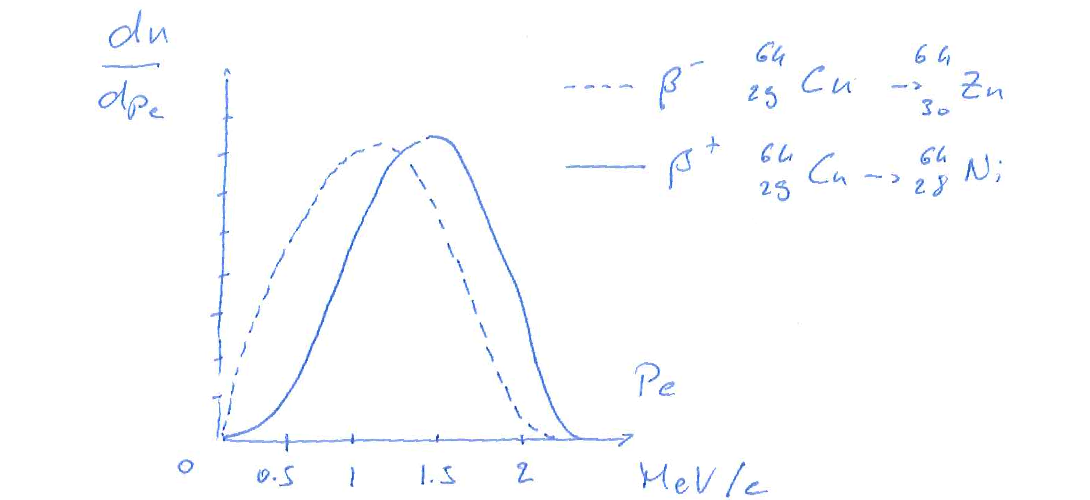
\includegraphics[scale=0.5]{Figures/nuclear-physics-fig20}
    \caption{Momentum distribution of the electron}
    \label{nuclear-physics-fig:20}
\end{figure}

This Coulomb correction can however be accurately calculated through a correction function $F(\pm Z, E_e)$, which looks significantly different for electrons and positrons, as illustrated in Figure \ref{nuclear-physics-fig:20}. Positrons tend to get higher momenta as they are repelled by protons in the nucleus, while the opposite happens for electrons.

The correction depends only on the charge of the nucleus and the energy available in the decay, $F(\pm Z, E_e)$, and therefore is a function of the kinetic energy of the electron.
One can therefore write the spectrum of emission of electrons/positrons as
\begin{equation*}
    \frac{1}{\lambda} \frac{d\lambda}{dT_e} \propto p_e (T_e+m_ec^2) p_\nu E_\nu F(\pm Z, T_e).
\end{equation*}

The decay probability can be evaluated through the following integral, where we have by hand inserted a factor $1/(m_ec^2)^5$ so that the factor is dimensionless:
\begin{equation*}
    f(Z,Q) = \frac{1}{(m_ec^2)^5}\int_0^Q p_e c (T_e + m_e c^2) p_\nu E_\nu F(\pm Z, T_e) \, dT_e,
\end{equation*}

This is often referred to as the \emph{Fermi function}, which is numerically estimated and tabulated and depends only on the charge of the nucleus and the energy of the $\beta$ decay $Q$.

Eventually, the decay rate can be written as
\begin{equation}
\label{BetaDecayRate}
    \lambda = \frac{G_F^2(m_ec^2)^5}{2\pi^3\hslash}|M_{fi}|^2 f(Z,Q).
\end{equation}


\subsection{The neutrino mass}
\label{sec:NeutrinoMass}
By analysing more closely the end-point of the distribution of the kinematic energy of the electron/positron in the $\beta$ decay \(N(A,Z)\to Y(A, Z+1)+e^-+\bar{\nu}_e\), we observe an interesting dependency at about
\begin{equation*}
    T_e^{max} = M(Z,A) - M(Z+1, A)- m_\nu = Q - m_\nu.
\end{equation*}
The energy spectrum is given by
\begin{equation*}
    \frac{d\lambda}{dT_e} = G_F^2 \frac{m_e^5c}{2\pi^3 \hslash} |M_{fi}|^2 F(\pm Z, T_e) p_e(m_ec^2 + T_e) (Q-T_e) \sqrt{(Q-T_e)^2 - m_\nu^2 c^4}
\end{equation*}
and therefore it depends on the mass of the neutrino. This dependence is usually looked at in terms of the \emph{Kurie plot} shown in Figure \ref{nuclear-physics-fig:21}, in which one plots the square root of the spectrum of the electron/positron kinetic energy (i.e. the number of electrons/positrons per bin of \(T_e\)), divided by the Fermi function, as a function of \(T_e\). The end-point of this spectrum is a measure of the electron neutrino mass: experiments typically observe few events in the Kurie plot, and so they are able to put an upper limit on the electron neutrino mass, rather than provide a measurement of its value.
\begin{figure}
    \centering
    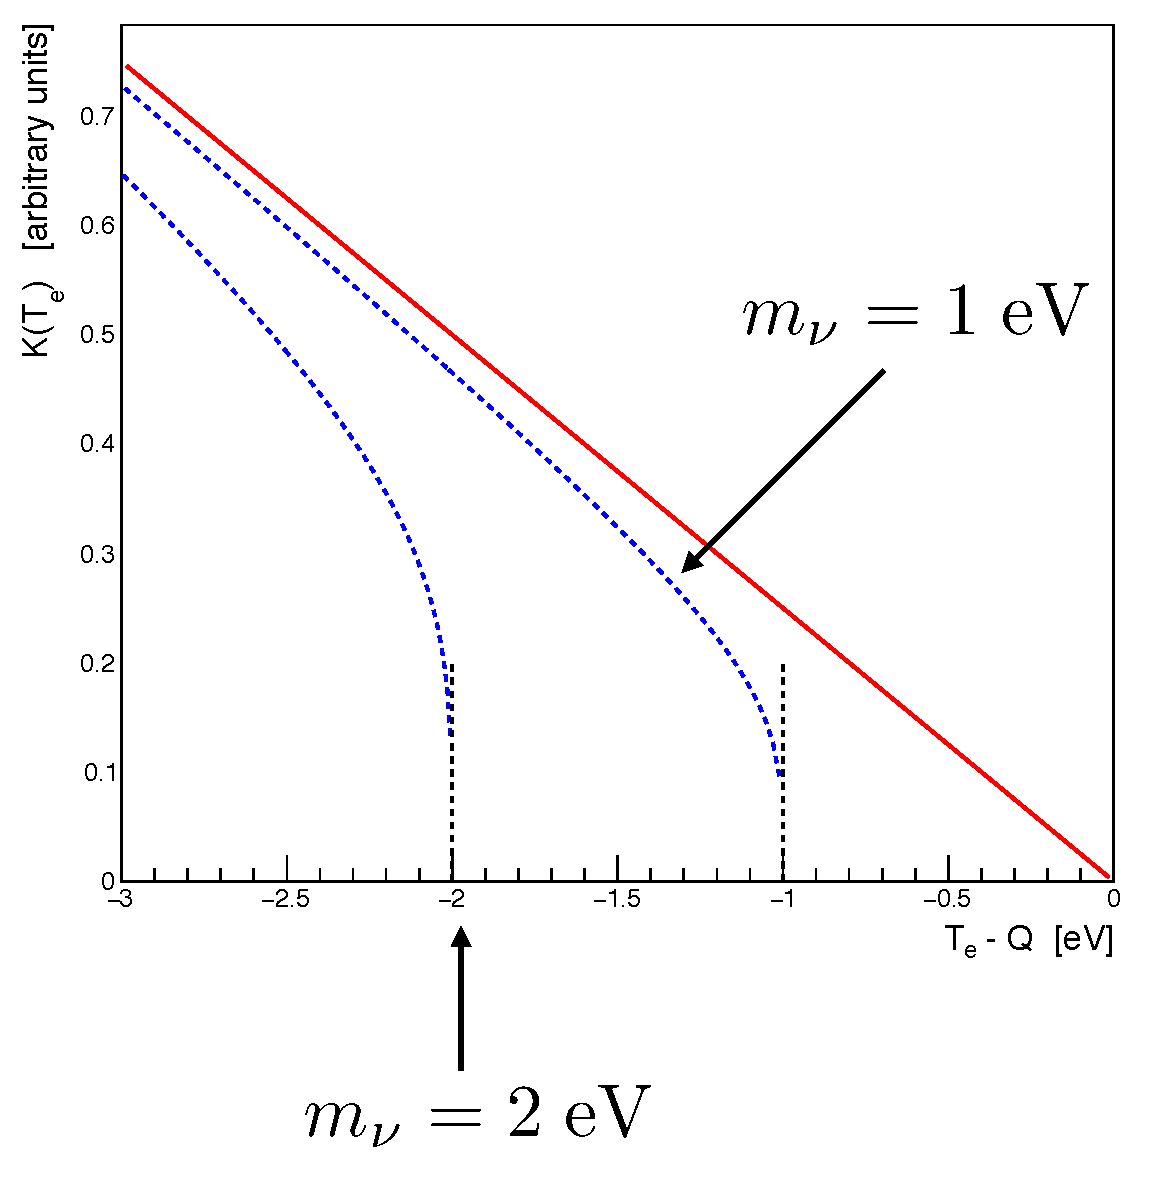
\includegraphics[scale=0.3]{Figures/nuclear-physics-fig21}
    \caption{End-point detail for the kinetic energy of electrons in a \(\beta^-\) decay, for different hypotheses on the neutrino mass.}
    \label{nuclear-physics-fig:21}
\end{figure}

Experimental constraints on the neutrino mass are obtained for example from \(\beta^-\) decays of \(H^3\) into \(He^3\) (\(Q = \SI{18.574}{keV}, T_{1/2}=\SI{12.3}{y}\)), and imply that \(m_{\nu_e}=m_{\bar{\nu}_e}\lesssim\SI{2}{eV}\).

\subsection{Sargent's law}
The element of rate \(d\lambda\) derived from the Fermi Golden rule in Eq.~\eqref{eq:ElementRate} can also be simplified assuming that the neutrino mass is negligible (a reasonable assumption given the experimental limits discussed in Section~\ref{sec:NeutrinoMass}). Then Eq.~\eqref{eq:ElementRate} can be rewritten as
\begin{eqnarray*}
    d\lambda & =& \frac{1}{2\pi^3\hslash^7 c^6} g^2|M_{fi}|^2 [ p_e c (W - E_e) \sqrt{(W - E_e)} E_e dE_e ] \\ 
    & = & \frac{1}{2\pi^3\hslash^7 c^6} g^2|M_{fi}|^2 \left[ p_e c (W - E_e)^2 E_e dE_e \right].
\end{eqnarray*}

If we integrate over all possible electron energies, and neglect the Fermi function, we get
\begin{equation}
        \lambda = \frac{1}{2\pi^3\hslash^7 c^6} g^2|M_{fi}|^2  \int_0^W  p_e c (W - E_e)^2 E_e dE_e \propto W^5.
\end{equation}
This leads us to define a useful rule for $\beta$ decays known as \emph{Sargent's law}: the overall rate of $\beta$ decays is proportional to the fifth power of the energy available to the decay.

\subsection{Interpretation}
\label{BetaInterpretation}
As was mentioned in the introduction of this section, $\beta$ decays have played a crucial role at many levels in Nuclear and Particle physics. The role of the large number of $\beta$ decay measurements of nuclei will be discussed in Section~\ref{sec:NuclearBeta}: here we will focus on what can be learned about the interaction underlying in $\beta$ decays.

It should first be said that it is through a thorough analysis of a large number of $\beta$ decays that a regular pattern could emerge, showing that there is a fundamental matrix element that can be factorised across all measurements done. We will illustrate this with only one example here, but there are many more (some discussed in Section~\ref{sec:NuclearBeta}).

As discussed in Section~\ref{sec:FermiTheory}, and as illustrated by Eq.~\eqref{eq:LExpansion}, the $\beta$ decays (or transitions) that are dominant are those corresponding to a vanishing angular momentum of the electron-anti-neutrino or positron-neutrino $\ell_{e\nu} = 0$ systems. These transitions are referred to as \emph{ allowed}, or in some cases \emph{ super allowed}, transitions. %This will be discussed a bit more in Section~\ref{sec:NuclearBeta}.
What ``allowed'' really means here is that it is the favoured process, as opposed to what will be referred to as  \emph{ forbidden} processes, corresponding to  $\ell_{e\nu} \geq 1$, which are disfavoured (``suppressed'').

Allowed decays ($\ell_{e\nu} = 0$) still correspond to a system of two particles (the electron and the neutrino) which are both fermions with spin \(1/2\). Therefore, if the neutron has spin up, for example, we can put the proton spin up or down, and this determines the total spin of the electron-neutrino system. From the composition of the electron and neutrino spins, we can identify two types of transitions which can occur, that characterize the electron-neutrino system and correspond to the two possible spin states $s_{e\nu} = 0$ (singlet anti-symmetric) and $s_{e\nu} = 1$ (triplet). The former kind of transition are referred to as \emph{Fermi transitions} and the latter as \emph{Gamow Teller} transitions. 

Depending on the nuclei involved in the $\beta$ decay, one or both are possible. A transition from a spin-zero state to another spin-zero state cannot be a Gamow Teller transition. Instead, a transition such as the neutron $\beta$ decay, which involves only spin-1/2 fermions, can have both types of transitions:
\begin{itemize}
    \item[-] {\bf Fermi} transitions for the neutron (antisymmetric singlet combination of the two spin-1/2 electron-neutrino system):
    
    $$ n\uparrow \rightarrow p\uparrow + \dfrac{1}{\sqrt{2}} \left [ (e^-\uparrow  \overline{\nu}_e \downarrow)  \, - \, (e^-\downarrow  \overline{\nu}_e \uparrow)  \right ] $$
    
        \item[-] {\bf Gamow Teller} transitions for the neutron (symmetric triplet combination of the two spin-1/2 electron-neutrino system):

  \begin{eqnarray}
  (s_{e\nu} = 0) & \; \; & n\uparrow \rightarrow  p\uparrow + \dfrac{1}{\sqrt{2}} \left [ (e^-\uparrow  \overline{\nu}_e \downarrow)  \, + \, (e^-\downarrow  \overline{\nu}_e \uparrow)  \right ] \; \; \; (m_s=0)\nonumber \\
    (s_{e\nu} = 1) & \; \; & \left \{ \begin{array}{cl}
    n\uparrow  \rightarrow  p\downarrow + e^-\uparrow  + \overline{\nu}_e \uparrow & \; \; \; (m_s =+1)  \\
    n\downarrow  \rightarrow  p\uparrow + e^-\downarrow  + \overline{\nu}_e \downarrow  & \; \; \; (m_s =-1) 
    \end{array} \right . \nonumber
  \end{eqnarray}  

\end{itemize}

One assumes that all the $\beta$ decays stem from an interaction with a given universal coupling constant, and that the differences in matrix element would come from simply counting the number of possible transitions (which thus rely on the spin combinations). In this case, the Gamow Teller matrix element should be three times larger than the Fermi transition matrix element. We then define the {\bf Fermi coupling constant} $G_F$ as the coupling corresponding to the Fermi transitions. The matrix element consists uniquely of a universal coupling constant $g$, as we have assumed in Eq.~\eqref{eq:ME-Fermi}, and $M_{fi}$ relates to the structure of the nucleus and its possible transitions (hence the name \emph{nuclear matrix element}).

The Fermi constant $G_F$ of Eq.~\eqref{eq:GF} can be interpreted as the constant that scales the Fermi transition for the neutron $\beta$ decay, or in general the constant that scales the Fermi transition matrix element (i.e. the one corresponding to the Fermi transitions of a nucleus, and not to the Gamow Teller ones). The reason for this is that, in the case of the neutron, there is only one possible configuration of the final state, and the corresponding matrix element can be considered as $|M_{fi}^F|^2 = 1$. Since for the Gamow Teller transitions there are three possible configurations, each reflecting a different $m_s$ for $s_{e\nu} = 1$, then the Gamow Teller matrix element will be $|M_{fi}^{GT}|^2 = 3$. In this case, and assuming no interference between the two processes, the overall matrix element can be written as
\[ |M_{fi}|^2 = |M_{fi}^F|^2 + \lambda^2 |M_{fi}^{GT}|^2,  \]
where the $\lambda^2$ factor gives the relative weight of the Gamow Teller transition matrix element: it is measured experimentally and its value is $\lambda = 1.24$. %We will come back to this and the estimate of the $\lambda$ factor in Section~\ref{sec:NuclearBeta} when discussing other types of transitions. \\

We can then take the estimated value of the $\lambda$ factor, the calculated effect of the Coulomb potential in the Fermi factor $f$, and the estimated matrix element, and measure the neutron lifetime $\tau = 890$~s to estimate  its $f\tau_{1/2} = 1.61 \times 10^3$~s. With all these ingredients, we can derive the Fermi constant, obtaining
\begin{equation*}
    G_F = 1.14 \times 10^{-5} \; \; {\rm GeV^{-2}}
\end{equation*}

The interpretation of these results in terms of fundamental interactions is made in Section~\ref{sec:WeakInteraction}.


\section{Gamma decays}

The $\gamma$ radioactive decay is an electromagnetic de-excitation process of the nucleus, which consists in the transition of a nucleus from an excited state to a lower energy state through the emission of a photon. In this sense this type of radioactivity is {\bf not} a decay and the nature and structure of the nucleus is unchanged. The $\gamma$ rays are more penetrating, but with much less ionizing power than the $\alpha$ and $\beta$ radiation. The $\gamma$ radiation occurs typically after $\alpha$ or $\beta$ decays, which leave the nucleus in an excited state and the emitted photons have discrete energies typically in the range from 100 keV to few MeV. \\

The emission of photons carries away angular momentum of the photon. This is a key observation for the construction of a model of nuclei. The fact that the $\gamma$ radiation is discrete suggests that the nucleus can be structure much like the atom is structured in energy shells with varying angular momenta. The emission of energetic photons can be viewed as the de-excitation of nuclei from a given initial excited state to a final state. \\

The theory of the $\gamma$ decays is based on the classification of the multi-pole transitions, both electric and magnetic, with the simplest one being the electric or magnetic dipoles.

\subsection{Dipole radiation}

The simplest example of the nuclear radiation can be computed from the Larmor formula, or the equivalent of the radiated power of an accelerated charge seen in Eq.~\ref{eq:AcceleratedChargePower} (see~\cite{jackson2} - page 664): 

\begin{equation}
\label{eq:Larmor}
    P = \dfrac{1}{12 \pi \varepsilon_0} \dfrac{\omega^4}{c^3} \vec{d}^2
\end{equation}

\noindent where $\vec{d} = e\vec{r} = \vec{d}_0 \sin \omega t$ represents the electric dipole of a charge $e$ and radius $\sim r$. The quantum mechanical version of the Larmor formula can be intuitively constructed from the classical formulation of Eq.~\ref{eq:Larmor} by replacing the dipole oscillation frequency $\omega$ by the radiated energy $E_{\gamma} = \hslash \omega$ and taking the classical dipole as an operator selecting specific quantified transitions from an initial state $\ket{i}$ to a final state $\bra{f}$ with a matrix element $\bra{f}\vec{d}\ket{i}$. Then the power can be expressed as follows:

$$ P =\dfrac{dE_{\gamma}}{dt} = \dfrac{1}{12 \pi \varepsilon_0} \dfrac{\omega^4}{c^3} \vec{d}^2 $$

\noindent from this expression we can obtain an intuitive formulation of the decay constant:

$$ \dfrac{1}{E_{\gamma}}\dfrac{dE_{\gamma}}{dt} = \lambda = 1/\tau = \dfrac{1}{\hslash \omega}\dfrac{1}{12 \pi \varepsilon_0} \dfrac{1}{\hslash}\dfrac{(\hslash \omega)^4}{(\hslash c)^3} |\bra{f}\vec{d}\ket{i}|^2$$

\noindent and therefore:

$$ \lambda = \dfrac{1}{12 \pi \varepsilon_0} \dfrac{1}{\hslash}\dfrac{E_{\gamma}^3}{(\hslash c)^3}  $$

\noindent as can intuitively be gathered from this expression is that it can be obtained as well through the Fermi golden rule! From this expression, with a $\gamma$ emitted with energy $E_{\gamma} = 1$~MeV from a nucleus with radius $R \sim 5$~fm we can infer that the corresponding lifetimes will be of the order of $10^{-6}$~s for an order of magnitude estimate and the following formula:

$$ \lambda \sim \dfrac{1}{3} \alpha E_{\gamma}^3 R^2 $$

\subsection{Magnetic dipole moment radiation}

Given the very small size of the nucleus 

Similarly to the electric dipole moment, a magnetic dipole radiates with an emitted power that follows the Larmor formula~\cite{jackson2}:

$$ P =\dfrac{dE_{\gamma}}{dt} = \dfrac{1}{12 \pi \varepsilon_0} \dfrac{\omega^4}{c^5} \vec{\mu}^2 $$

With the same intuitive calculation done above, and considering a typical nuclear magnetic moment, referred to as nuclear magneton: 

$$ \mu_N = \dfrac{e \hslash}{2 m_p} $$

Comparing to the previous formula one gets a ratio of the decay constants for the magnetic dipole moment $\lambda_M$ to that for the electric dipole moment $\lambda_E$ of:

$$ \frac{\lambda_M}{\lambda_E} \sim \left ( \dfrac{e\hslash}{2m_p} \right )^2 \dfrac{1}{(eR)^2} = 10^{-3}$$

\subsection{Multipole radiation}

Similarly to the case of the Fermi theory for the $\beta$ decay, in the case of the photon emission, the photon can carry away off the nucleus higher angular momentum than only that corresponding to its spin i.e $\ell =1$. The magnetic and electric dipole radiations correspond to an orbital momentum of the photon the is equal to 0. Higher angular momenta can be carried away from multipole radiation. Multipole radiation can be treated in a similar way as expressed above for the dipole radiations. It is interesting to note that in terms of orders of magnitude, the rate of the electric quadrupole pole radiation is $10^{-3}$ smaller than the dipole radiation, and thus similar to the magnetic dipole radiation. Then the octupole radiation is $10^{-3}$ smaller than the dipole radiation, and of the same order as the magnetic quadrupole radiation and son on.

\subsection{Internal conversions}

finally another interesting process can occur for excited nuclei that can undergo $\gamma$ radiation, is the so-called {\bf internal conversion} process. This process corresponds to the emission of an electron without any transmutation of the emitting nuclei (therefore not corresponding to a $\beta$ decay). It occurs for atomic nuclei where an electron from an atomic inner layer, has a non vanishing probability to penetrate the volume of the nucleus. When the nucleus is in an excited state which could undergo a $\gamma$ emission, it is the electron which through the coupling to the excited nucleus is emitted with a kinetic energy corresponding to the $\gamma$ transition energy in the nucleus to which the atomic binding energy of the electron has to be subtracted.

\subsection{Interpretation and selection rules}

As has been discussed in the introductory remarks of this section, the observation of $\gamma$ emission with a discrete spectrum is an essential feature to further understand the how nuclei are structured. These aspects will be discussed in more detail in chapter~\ref{chapter-nuclear-physics}, when building a shell model of the nucleus. \\

%%% Local Variables:
%%% mode: latex
%%% TeX-master: "../book"
%%% End:

% LocalWords: Springer

%%% Problema completo

\section{Problems}

\begin{prob}\label{prob1}

Nel 1947, Enrico Fermi intraprese la costruzione di un acceleratore di protoni, detto ciclotrone, alla frontiera in energia: questo
ciclotrone, che accelerava protoni ad un'energia cinetica di
\SI{450}{MeV}, fu per breve tempo l'acceleratore di più alta energia
al mondo. Fermi e i suoi collaboratori usarono un bersaglio mobile,
che permetteva così di ottenere collisioni di diverse energie. Una
targhetta di Berillio permetteva di produrre pioni, e in particolare
pioni negativi $\pi^-$ selezionati, come in figura per avere energie
diverse. Il fascio di pioni veniva successivamente mandato su una
targhetta di idrogeno liquido. La Figura~\ref{Setup} rappresenta
l'apparato sperimentale.

\begin{figure}[ht]
%\centering
%\includegraphics[width=0.75\textwidth]{Setup.pdf}
\vskip -0.2cm
\caption{\label{Setup} L'apparato sperimentale del Ciclotrone di
  Chicago, e illustrazione della produzione del fascio di $\pi^-$ e
  del apparato di rivelazione.}
\end{figure}


\begin{enumerate}

\item La distanza fra il bersaglio e il centro del ciclotrone è di 76
  pollici (cioè \SI{1.90}{m}). Qual è il campo magnetico B necessario
  ad ottenere protoni con un'energia cinetica di \SI{450}{MeV}?

\item Quale è l’energia nel centro di massa della reazione $\pi^- p$
  per un fascio di pioni negativi con un'energia cinetica di
  \SI{100}{MeV}?

\item Che energia cinetica devono avere i pioni per produrre la
  risonanza $\Delta^0$ di massa 1232~$\rm MeV/c^2$?



\item Considerando pioni con energia cinetica sufficiente per produrre
  la risonanza $\Delta^0$, nella reazione $\pi^- p \rightarrow \pi^0 n$
  quali sono l'energia minima e massima del $\pi^0$ nel laboratorio?

%\item Il pione neutro $\pi^0$ decade in due fotoni. Quale \`e nel
%  sistema di riferimento del laboratorio l'angolo minimo tra i due
%  fotoni quando il pione ha il massimo di energia nella resazione? E
%  quando \`e al minimo di energia? Quale è l'angolo massimo di
%  apertura tra i fotoni in entrambi casi?
\end{enumerate}

{\it Dati} $m_{\pi^{\pm}} = 140$~MeV/c$^2$,  $m_{\pi^0} = 135$~MeV/c$^2$, $m_{p} = 938$~MeV/c$^2$ e $m_{n} = 940$~MeV/c$^2$


\end{prob}


\section*{Take-home lessons}
\begin{itemize}
    \item Both nuclei and particles (whether elementary or not) decay. Decays are random processes which are denoted by a given decay probability, which is a property of the decaying particle. The ratio between the decay probability and the decay time does not depend on time, and the decay probability of a single particle in a set of $N$ particles does not depend on $N$.
    \item The description of metastable systems in the time-independent scattering theory allows to express the cross-section of a decay process as in the case of a dumped harmonic oscillator. The mean lifetime $\tau$ of a particle is related to its total decay width $\Gamma$ via the relation $\Gamma = \hslash/\tau$. The probability of having a particle with a given energy is given by the Breit-Wigner formula.
    \item The kinematics of $\alpha$, $\beta$, and $\gamma$ decays can be described introducing the disintegration energy $Q$, defined as the sum of the kinetic energies of the decay particles.
    \item The number of radioactive atoms in a system can be increased -- for example, due to spallation reactions, where incoming particles collide with atomic nuclei and produce lighter particles, or due to chain decays. The number of radioactive atoms has an equilibrium condition, in which the relative concentration of different elements is equal to the ratio of their mean lifetimes (\emph{secular equilibrium}).
    \item In the case of $\alpha$ decays, there is an empirical relation between the half-life of a decay and its disintegration energy $Q$, given by the Geiger-Nuttal law, $\ln t_{1/2}=a+b/\sqrt{Q}$. Gamow's model of $\alpha$ decays is able to explain this law: the $\alpha$ particle is assumed to be confined in a well by a potential generated by the nucleus, with a non-zero probability to cross the potential barrier and reach a region of Coulomb potential. The tunneling probability is calculated by treating the potential barrier as a series of infinitesimal barriers, i.e. the overall tunneling probability is given by the product of the infinitesimal probabilities, $P\propto e^{-2G}$, where $G$ is the Gamow factor. The Gamow factor can be calculated and used to determine the mean lifetime, which has the same dependence on $Q$ as in the Geiger-Nuttal law.
    \item There are three kinds of $\beta$ decays: $\beta^-$ decays in which a neutron in an atom converts to a proton with the emission of an electron, $\beta^+$ decays in which a proton converts to a neutron with the emission of a positron, and electron capture, in which a proton converts to a neutron by capturing an atomic electron. Contrary to $\alpha$ decays, $\beta$ decays are not two-body decays, as determined by looking at the experimental energy spectrum (which isn't monochromatic). One has to then consider the decay as a three-body decay, e.g. $n\to p e \bar{nu}_e$ in the $\beta^-$ decay, where a new particle, the anti-neutrino $\bar{\nu}_e$, has to be introduced. The neutrino and the anti-neutrino have spin $1/2$, as required by the conservation of angular momentum. The Fermi theory of $\beta$ decays introduces a new, short-range interaction (a \emph{contact interaction}) which is able to create or absorb fermions. The calculation of the decay cross-section is complicated by the need to take into account all possible combinations of momenta in the three-body decay to compute the density of states. The resulting decay rate must be corrected for the effect of the electrostatic field of the nucleus on the momentum of the emitted electron or positron, which is expressed by the Fermi function as a function of the atomic number of the nucleus and of the electron energy. The resulting energy spectrum has an endpoint which depends on the neutrino mass: if the mass is neglected, the decay rate is proportional to the fifth power of the energy available to the decay (\emph{Sargent's law}).
    \item The $\gamma$ decay corresponds to an electromagnetic de-excitation of the nucleus, which transitions from an excited state to a lower-energy state by emitting a photon. Strictly speaking, the nucleus does not change nature, so the process isn't technically a decay. The emitted photon carries away the angular momentum of the nucleus: from the experimental fact that $\gamma$ radiation is discrete in energy, one can deduce a structure of the energy levels of the nucleus similar to the one of atoms. The theory of $\gamma$ decays is based on the classification of multi-pole transitions (electric and magnetic).
\end{itemize}
\section*{Questions}
\begin{itemize}
    \item Why should the neutrino have spin $1/2$?
\end{itemize}
